\documentclass[11pt]{article}

% ---------------------------------------------------------------- packages
\usepackage[margin=1.05in]{geometry}
\usepackage[utf8]{inputenc}
\usepackage[T1]{fontenc}
\usepackage{lmodern}
\usepackage{microtype}
\usepackage{amsmath,amssymb,amsthm,mathtools}
\usepackage{booktabs,array,multirow,longtable}
\usepackage{xcolor}
\usepackage{tikz}
\usepackage{pgfplots}
\pgfplotsset{compat=1.17}
\usepackage[numbers,sort&compress]{natbib}
\usepackage[hidelinks]{hyperref}
\usepackage[capitalise]{cleveref}

% ---------------------------------------------------------------- macros
\newcommand{\F}{{\mathbb{F}_2}}
\newcommand{\MM}[3]{\langle #1,#2,#3\rangle}
\newcommand{\rk}{\operatorname{rk}}
\newcommand{\todo}[1]{{\color{red}[TODO: #1]}}

% ---------------------------------------------------------------- front matter
\title{Upper Bounds on the GF(2) Rank of Matrix Multiplication\\
Below Four Public Tables: 795 Formats up to $32\times32\times32$\\
and a Prior-Art Check}
\author{Erik Peterson\thanks{\todo{affiliation and contact e-mail}}}
\date{\today\ \textbf{(draft)}}

\begin{document}
\maketitle

\begin{abstract}
We report exact decompositions of the matrix-multiplication tensor over $\mathrm{GF}(2)$ for 795 formats $\MM nmp$ with all sides at most 32 whose rank is below every rank that four public tables list on 2026-09-29, in any ring (733 formats) or among schemes known to be valid over $\F$ (62 formats). They are upper bounds only.
The tables omit public GF(2)-valid prior art, and a check against the literature shows it: 87 of the 795 are superseded by published constructions or claims (80 by schemes we rebuilt and verified, 7 by published rank claims that we did not reproduce) and 112 more equal the rank of a composition of published schemes; 596 remain.
Most of the 795 have no walk and no projection in their recorded lineage (507: 379 compositions, and 128 certificates and fleet checkpoints of earlier stages, which include walks); the rank-47 scheme for $\MM444$ over $\F$ is the most frequent ingredient, and 92\% have a side above 16.
For the 733 strongest the median saving over the listed rank is 29 terms (0.9\%); the largest are 268 terms, for $\MM{20}{23}{32}$ (7{,}772 against 8{,}040), and 4.8\%, for $\MM{15}{16}{17}$, and both remain. Neither record with all sides at most 8 is new.
The comparison is easy to overstate (458 of the 733 have no GF(2)-valid scheme listed at all, commutative algorithms must be excluded, and the tables move), so we describe it carefully.
All tensors are exact over $\F$ and were checked by two separately written implementations; 691 ship with their derivation. The methods are in a companion paper.
\end{abstract}

\noindent\textbf{Keywords:} matrix multiplication, tensor rank, bilinear algorithms, $\mathrm{GF}(2)$, upper bounds.\\
\textbf{MSC 2020:} 68Q25, 15A69, 68W30.

\section{Introduction}\label{sec:intro}

The rank of the matrix-multiplication tensor $\MM nmp$ over a field bounds the number of multiplications of any bilinear algorithm for $n\times m$ by $m\times p$ products over that field \cite{burgisser1997algebraic,landsberg2012tensors}.
Over $\F$ there are schemes that have no counterpart in other characteristics, the rank-47 scheme for $\MM444$ being the best known \cite{fawzi2022discovering}, and flip-graph searches have since improved several small formats over $\F$
\cite{kauers2023flip,kauers2022still,arai2024adaptive,moosbauer2025flip,kauers2025meta,medley2026gpu}.
Two public tables list a rank for every format up to $32\times32\times32$ \cite{sedoglavic2026catalogue,lacelle2026catalog}, and two repositories hold explicit schemes for formats with all sides at most $16$ \cite{perminov2026fmmrepo,witteveen2026schemes} (the second only 25 of them), but these tables were built for arbitrary rings;
for most large formats the listed rank is obtained by composing smaller schemes, and these compositions generally do not use the schemes that are best in characteristic two (for $\MM448$ the catalogue's minimum among schemes stamped F2 is 96, although it lists the F2 rank-47 scheme for $\MM444$).

In September 2026 we built a pipeline that composes, projects and walks over $\F$ (described in a companion paper \cite{peterson2026methods}) and compared its output, and the output of two earlier stages of the same project, with four public tables.
This paper reports the outcome as a list of exact schemes, and analyses it.
For each of 795 formats with all sides at most 32, the best scheme we hold has smaller rank than every entry of the tables for that format in any ring (733 formats) or smaller than every listed scheme known to be valid over $\F$ (62 formats).
The tables are not the whole of the public record, however: a check against the literature (\cref{sec:persistence}) finds published constructions and claims that supersede 87 of these 795 and constructions that equal the rank of 112 more, leaving 596.

\paragraph{Summary.}
\begin{itemize}
\item The records are exact: every tensor was expanded against the full matrix-multiplication tensor by two separately written implementations, and 691 of the 795 are accompanied by their derivation (\cref{sec:verification}).
\item The tables omit public prior art. Published GF(2)-valid schemes that they lack, rank claims kept in the matmulcatalog's own \texttt{cited-bounds} file, and compositions of listed schemes supersede 87 of the 795 (which we withdraw; for seven of them only a published claim, which we did not reproduce) and match 112 more; 596 remain (\cref{sec:persistence}).
\item They are concentrated in large formats: 734 of 795 have a side above 16, and only 61 have all sides at most 16. Every format with all sides at most 16 has a verified scheme, so the concentration is about where improvements exist, not only about where we looked (\cref{sec:overview}).
\item Most have no walk and no projection in their recorded lineage (507 of 795): 379 are compositions whose rank follows from the ranks of their parts (block sums, Kronecker products, block recombinations, replayed catalogue recipes), and 128 are certificates and fleet checkpoints of earlier stages of the project, which include walks. The 4$\times$4$\times$4 rank-47 scheme is a leaf of 58 of the 203 pure closure products and the outer scheme of the July block compositions.
Walks and projections are part of the lineage of 288 records (\cref{sec:nature}).
\item Margins are modest: for the 733 records below every listed rank the median saving over the best listed rank is 29 terms (0.91\%; 26 terms over all 795 against the bar that defines each class); the largest are 268 terms ($\MM{20}{23}{32}$) and 4.8\% ($\MM{15}{16}{17}$); 59 of the 733 beat the listed rank by exactly one.
The best normalized exponent among the records is 2.7870 ($\MM{15}{16}{16}$ at rank 2{,}137), worse than that of $\MM444$ at rank 47 (2.7773; \cref{sec:highlights}).
\item The comparison is delicate. Of the 733 strongest records, 458 have no GF(2)-valid scheme listed at all; commutative algorithms must be excluded (a commutative entry lies at or below our rank for five records); all four tables changed during the campaign; and preprints report rank 94 for $\MM448$ over $\mathbb Z_2$ \cite{perminov2025ternary} and rank 245 for $\MM777$ over $\F$ \cite{medley2026gpu}, so neither of our two records with all sides at most 8 is new (\cref{sec:comparators,sec:persistence}).
\end{itemize}

\paragraph{How to read these results.}
Three qualifiers apply throughout. First, every rank is an upper bound; we prove no lower bound. Second, ``record'' means smaller than the entries of four tables at stated revisions; it does not mean new to the literature, and following the project's claim policy we call each result \emph{apparent} until a complete prior-art audit has been done; the check of \cref{sec:persistence} is not that audit, and it already removes 87 records and reclassifies 112.
Third, many of the results are best understood as the completion over $\F$ of constructions that the tables already contain over other rings: replacing a leaf of a known composition by its better $\F$ counterpart lowers the rank of every format that uses it.
That is worth recording, and it is how 203 of the records arise (75 of them remain after the check of \cref{sec:persistence}), but it is not the same kind of result as a new scheme for a small format.

\paragraph{Organization.}
\Cref{sec:setting} fixes the setting and definitions, \cref{sec:overview} gives the counts, \cref{sec:nature} analyses how the records arose, \cref{sec:highlights} lists notable ones, \cref{sec:comparators} examines the comparison in detail, \cref{sec:persistence} reports a re-scoring against later table revisions and a literature check,
\cref{sec:verification} summarizes verification and \cref{sec:limits} states limitations and data availability. The full list is in \cref{app:all}.

\section{Setting and definitions}\label{sec:setting}

\paragraph{Schemes and formats.}
A scheme of rank $r$ for $\MM nmp$ over $\F$ is a list of $r$ triples $(u_t,v_t,w_t)$ of nonzero bit vectors of lengths $nm$, $mp$, $np$ with
$\sum_t u_t\otimes v_t\otimes w_t=\sum_{i,j,k}e_{(i,j)}\otimes e_{(j,k)}\otimes e_{(i,k)}$ over $\F$; it computes $(AB)_{ik}=\sum_t w_t[(i,k)]\langle u_t,A\rangle\langle v_t,B\rangle$ with $r$ multiplications.
The rank depends only on the multiset $\{n,m,p\}$, so we index everything by \emph{sorted} formats $n\le m\le p$; a scheme for one ordering yields one for every ordering by permuting coordinates.
The universe here is the 5{,}456 sorted formats with all sides between 2 and 32; 3{,}662 of them (67.1\%) have a verified scheme in our holdings, including all 680 formats with all sides at most 16.
Each sorted format stands for up to six orderings: the 3{,}662 formats represent 20{,}217 of the 29{,}791 ordered formats, and the 795 records represent 4{,}343.

\paragraph{The four tables.}
\Cref{tab:sources} lists the sources against which every result is compared, at the revisions pinned on the day of scoring.
The Lille digest records only a rank and an exponent per sorted format, with no coefficient field or ring; the matmulcatalog records the fields over which each scheme is valid and flags commutative algorithms;
the FastMatrixMultiplication repository and the fmm-schemes dataset store coefficients (rings ZT $=\{-1,0,1\}$, Z and Q), from which the ring can be read.
\begin{table}[t]
\centering\small
\begin{tabular}{@{}p{4.0cm}p{4.5cm}p{2.3cm}p{1.9cm}@{}}
\toprule
source & lists & revision & date\\
\midrule
Lille digest \cite{sedoglavic2026catalogue} & rank and exponent per sorted format up to 32 (no field) & \texttt{9f26324} & 2026-09-28\\
matmulcatalog \cite{lacelle2026catalog} & schemes with the fields they are valid over; commutative algorithms flagged & \texttt{f0c2ba9} & 2026-09-29\\
FastMatrixMultiplication \cite{perminov2026fmmrepo} & ZT, Z and Q schemes, formats up to 16 (ring in the file name) & \texttt{613599b} & 2026-09-28\\
fmm-schemes \cite{witteveen2026schemes} & 25 ZT schemes, sides at most 16 (largest volume $13\times14\times16$) & \texttt{8fa0f2a} (release 1.1) & 2026-09-27\\
\bottomrule
\end{tabular}
\caption{The four tables and the revisions scored against.}
\label{tab:sources}
\end{table}

\paragraph{Bars and classes.}
For a sorted format $s$, the \emph{any-ring bar} $B_{\mathrm{any}}(s)$ is the least rank listed by any source (commutative algorithms excluded), and the \emph{GF(2)-valid bar} $B_{\F}(s)$ is the least rank among matmulcatalog entries whose field list contains F2 and among ZT and Z schemes of the two repositories, which reduce modulo two; rational (\texttt{Q}) schemes never count, and the files under \texttt{schemes/known/} of the FastMatrixMultiplication repository are not read (reading them would change no class). The bar is undefined when nothing GF(2)-valid is listed.
A verified scheme of rank $r$ for $s$ is \textsf{below\_all} if $r<B_{\mathrm{any}}(s)$; otherwise \textsf{gf2\_valid\_only} if $r<B_{\F}(s)$; otherwise a \textsf{tie} if $r=B_{\mathrm{any}}(s)$ and \textsf{above} if not.
A \emph{record} is a format whose best scheme is \textsf{below\_all} or \textsf{gf2\_valid\_only}. On the scoreboard of 2026-09-29 there are 733 and 62 of these; 1{,}413 formats tie and 1{,}454 are above (\cref{tab:classes}).
The definitions and the pitfalls of this comparison are treated in \cref{sec:comparators} and in the companion paper.

\paragraph{Holdings.}
The scoreboard keeps, per sorted format, the lowest-rank scheme among all exact files found in the campaign's working directories, the committed certificates of the package, its packaged seeds and the live fleet's checkpoints; a file counts only if it passes the exactness gate, and verdicts are cached by content hash.
Ties in rank keep the lexicographically first path, so a record is one particular tensor of that rank, identified by its SHA-256; the index gives the hash of one exact tensor of that rank held in the release, which for 18 rows is an equal-rank sibling of the file the scoreboard chose.

\section{Overview of the results}\label{sec:overview}

\paragraph{Counts.}
\Cref{tab:classes} gives the classification of the 3{,}662 formats for which we hold a verified scheme. Of these, 795 are records: 733 below every listed rank in any ring, and 62 below every listed GF(2)-valid rank while another table lists an equal or lower rank for an unspecified or different field.
\begin{table}[t]
\centering\small
\begin{tabular}{@{}lr@{}}
\toprule
class of the best verified scheme of a sorted format & formats\\
\midrule
\textsf{below\_all}: below every listed rank in any ring & \textbf{733}\\
\textsf{gf2\_valid\_only}: below every listed GF(2)-valid rank only & \textbf{62}\\
\textsf{tie}: equal to the best listed rank & 1{,}413\\
\textsf{above}: above the best listed rank & 1{,}454\\
\midrule
formats with a verified scheme (of 5{,}456) & 3{,}662\\
\bottomrule
\end{tabular}
\caption{Classification of the scoreboard of 2026-09-29 against the four tables of \cref{tab:sources}.}
\label{tab:classes}
\end{table}

\paragraph{Where the records are.}
Records are overwhelmingly formats with a large side (\cref{tab:size,fig:maxside}): 734 of the 795 (92.3\%) have a side above 16 and 61 have all sides at most 16; only 9 have all sides at most 12 and 2 at most 8.
The share of verified formats that are records is 2--4\% for maximum side up to 12, 13\% for 13--16, and 24.6\% above 16.
\begin{table}[t]
\centering\small
\begin{tabular}{@{}lrrrrrr@{}}
\toprule
largest side & \textsf{below\_all} & \textsf{gf2\_valid\_only} & records & verified formats & universe & records/verified\\
\midrule
2--8 & 2 & 0 & 2 & 84 & 84 & 2.4\%\\
9--12 & 5 & 2 & 7 & 202 & 202 & 3.5\%\\
13--16 & 34 & 18 & 52 & 394 & 394 & 13.2\%\\
17--24 & 263 & 15 & 278 & 1{,}129 & 1{,}620 & 24.6\%\\
25--32 & 429 & 27 & 456 & 1{,}853 & 3{,}156 & 24.6\%\\
\midrule
all & 733 & 62 & 795 & 3{,}662 & 5{,}456 & 21.7\%\\
\bottomrule
\end{tabular}
\caption{Records by largest side. Every format with all sides at most 16 has a verified scheme; above 16 we hold schemes for 70\% and 59\% of the formats.}
\label{tab:size}
\end{table}

\begin{figure}[t]
\centering
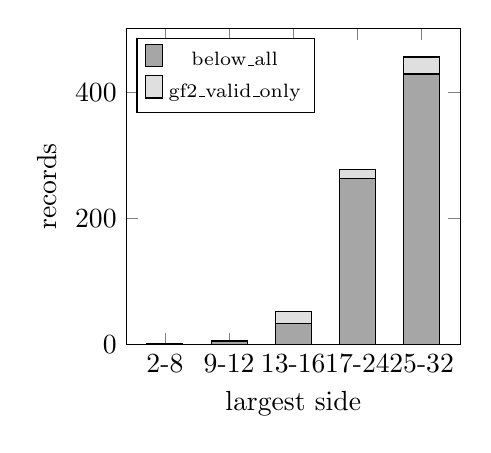
\begin{tikzpicture}
\begin{axis}[ybar stacked,width=0.48\textwidth,height=5.6cm,bar width=13pt,ymin=0,
  symbolic x coords={2-8,9-12,13-16,17-24,25-32},xtick=data,xlabel={largest side},ylabel={records},
  legend style={at={(0.03,0.97)},anchor=north west,font=\scriptsize},enlarge x limits=0.15]
\addplot[fill=gray!70] coordinates {(2-8,2) (9-12,5) (13-16,34) (17-24,263) (25-32,429)};
\addplot[fill=gray!25] coordinates {(2-8,0) (9-12,2) (13-16,18) (17-24,15) (25-32,27)};
\legend{below\_all,gf2\_valid\_only}
\end{axis}
\end{tikzpicture}\hfill
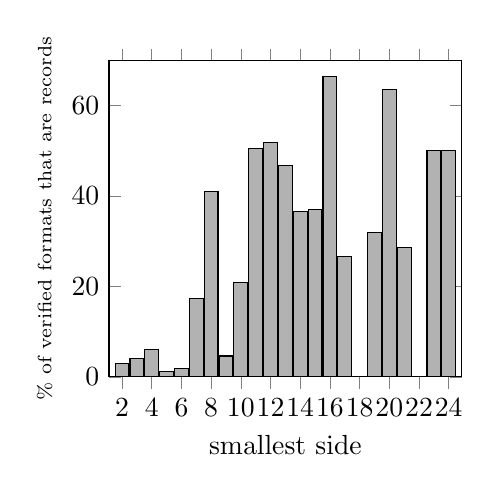
\begin{tikzpicture}
\begin{axis}[ybar,width=0.5\textwidth,height=5.6cm,bar width=5pt,ymin=0,ymax=70,
  xtick={2,4,6,8,10,12,14,16,18,20,22,24},xlabel={smallest side},ylabel={\% of verified formats that are records},
  ylabel style={font=\scriptsize},enlarge x limits=0.04]
\addplot[fill=gray!60] coordinates {(2,3.0) (3,4.0) (4,6.0) (5,1.1) (6,1.8) (7,17.4) (8,40.9) (9,4.6) (10,20.9) (11,50.5) (12,51.8) (13,46.8) (14,36.6) (15,37.1) (16,66.4) (17,26.7) (18,0) (19,32.0) (20,63.5) (21,28.6) (22,0) (23,50.0) (24,50.0)};
\end{axis}
\end{tikzpicture}
\caption{Left: records by largest side. Right: the share of verified formats that are records, by smallest side (smallest sides 25--28 have 4--8 verified formats each, and none above 28).}
\label{fig:maxside}
\end{figure}

The right panel of \cref{fig:maxside} shows how the records depend on the smallest side: they are rare when it is between 2 and 6 (1--6\%), common between 11 and 16 (37--66\%), and irregular above 16 where few formats have been verified; there are dips at 9 (4.6\%) and 18 (none of 39 verified formats) and peaks at 8, 11--13, 16 and 20. We did not investigate the pattern; it is what one expects if improvements come from composing blocks of a few favourable sizes.

\paragraph{New and old.}
The scoreboard held 560 records on the morning of 2026-09-29 (533 \textsf{below\_all}, 27 \textsf{gf2\_valid\_only}) against the same tables. During the day 235 formats became records (200 and 35), 49 earlier records were lowered further (by 1{,}513 terms in total; median 22, at least 10 for 37 of them), and none was lost;
182 of the 235 new records are formats for which we had no verified scheme in the morning, and coverage of the universe rose from 31.2\% to 67.1\%.
Of the 560 earlier records, 189 descend from the July block-composition certificates, 140 from certificates committed 2026-09-22 to 09-26, 183 from closure products of the first days of the campaign, 40 from matmulcatalog replays, and 8 from public seeds and the project's live fleet; of the 235 new ones, 149 descend from closure products, 55 from replays and 31 from July or committed certificates.

\section{How the records arose}\label{sec:nature}

Each record is one tensor, and for 691 of the 795 the data release records its lineage: a seed and the chain of steps that led from it to the retained scheme (for the 102 committed certificates that stay in the repository the steps are documented in their certificate directories, and the two fleet checkpoints have no recorded lineage). \Cref{tab:families} groups the 795 by lineage family; the codes are defined in \cref{app:families}.

\begin{table}[t]
\centering\small
\begin{tabular}{@{}p{7.4cm}lrrrr@{}}
\toprule
lineage of the recorded tensor & code & records & new on 09-29 & \multicolumn{2}{c}{median saving}\\
& & & & terms & \%\\
\midrule
closure product (block sums and Kronecker products of exact schemes) & C & 203 & 52 & 16 & 0.74\\
July 2026 block-composition certificate & J & 152 & 0 & 50 & 1.81\\
certificate committed 2026-09-22 to 09-26 & K & 126 & 0 & 50 & 1.33\\
closure product, projected and walked (in several rounds) & CPW & 106 & 85 & 34 & 1.01\\
replayed recipe, then walked & MW & 58 & 38 & 2 & 0.08\\
July certificate, projected & JP & 36 & 0 & 19.5 & 0.74\\
matmulcatalog recipe replayed over $\F$ & M & 24 & 4 & 3 & 0.14\\
committed certificate, projected and walked & KPW & 23 & 14 & 36 & 0.87\\
July certificate, projected and walked & JPW & 15 & 14 & 12 & 0.38\\
closure product, then projected & CP & 15 & 5 & 30 & 1.61\\
replayed recipe, projected and walked & MPW & 12 & 12 & 10.5 & 0.43\\
closure product, then walked & CW & 8 & 7 & 5.5 & 0.13\\
committed certificate, projected & KP & 8 & 3 & 18.5 & 0.74\\
public integer scheme reduced mod 2, then walked & S & 6 & 0 & 1.5 & 0.15\\
live-fleet construction/checkpoint & F & 2 & 0 & 27 & 1.66\\
replayed recipe, then projected & MP & 1 & 1 & 10 & 0.56\\
\midrule
all & & 795 & 235 & 26 & 0.91
\\
\bottomrule
\end{tabular}
\caption{Records by lineage family. ``Saving'' is the listed rank minus ours, against the bar that defines the record's class (any-ring for the 733 strongest, GF(2)-valid for the 62 others). Families whose names contain ``walked'' contain at least one walk; ``projected'' at least one projection. Two rows of the archive's index labelled ``live fleet checkpoint'' are corrected here: the tensor recorded for $\MM999$ is a walk from a public scheme and the one recorded for $\MM{13}{13}{13}$ is a July composition.}
\label{tab:families}
\end{table}

\paragraph{Most records have no walk or projection in their recorded lineage.}
507 of the 795 records (63.8\%) have no walk and no projection in the lineage recorded for them: 203 closure products, 152 July certificates, 126 certificates committed on 2026-09-22 to 09-26, 24 matmulcatalog recipes replayed over $\F$ and two records of the project's live fleet.
For 379 of them (the closure products, the July certificates and the replays) the rank follows from the ranks of components by arithmetic: sums and products of ranks, less the terms that vanish or cancel when the parts are assembled.
The 126 committed certificates and the two fleet records are different: they are outputs of earlier stages of the project, including walks. The steps of the committed certificates are documented in the repository's certificate directories and not in the lineage of this release (see below); the two fleet checkpoints ($\MM777$, from a July construction, and $\MM{15}{15}{15}$, from a July composition by the fleet's walkers) have no recorded lineage.
The saving is large where the composition is deep (median 50 terms for the July and the committed certificates, 16 for the closure products) and small where a single recipe is replayed (3 terms).
The most frequent component is the rank-47 scheme for $\MM444$ of Fawzi et al.\ \cite{fawzi2022discovering}, in the presentation packaged with the tools: it is a leaf of 58 of the 203 closure products, in 55 of its 59 uses as a Kronecker factor, and the July block compositions use it as their outer scheme.

\paragraph{Where the roots are.}
Counted by the earliest stage in the lineage, 360 records (45.3\%) descend from the July and the committed certificates (203 and 157, with their projections and walks), 332 (41.8\%) from closure products, 95 (11.9\%) from replayed matmulcatalog recipes and eight from public seeds and the live fleet.
The 795 are therefore the pooled results of three stages of one project (July 2026, 2026-09-22 to 09-26, and the campaign of the companion paper \cite{peterson2026methods}), not the yield of the last four days alone.

\paragraph{Block recombination with the rank-47 scheme.}
The July certificates, and the committed certificates that descend from them, come from one construction that is not new: support-aware block recombination, in the form implemented by the public AlphaTensor code, which credits Sedoglavic's $7\times7$ construction \cite{sedoglavic2017seven} and Drevet et al.\ \cite{drevet2011optimization} for the idea.
Let $\sum_{t=1}^{47}U_t\otimes V_t\otimes W_t$ be the rank-47 scheme for $\MM444$ over $\F$ and cut $n$, $m$ and $p$ each into four parts of possibly different sizes. Term $t$ multiplies a sum of blocks of $A$ by a sum of blocks of $B$ and adds the product to blocks of $C$.
After zero-padding the blocks to a common size, only the leading $s_n\times s_m$ corner of the first sum and the leading $s_m\times s_p$ corner of the second can be nonzero, and only the leading $s_n\times s_p$ corner of the product is used; each of the three sizes is the smaller of the largest parts touched by the two factors that share the axis. Hence
\[
  \operatorname{rk}\MM nmp\;\le\;\sum_{t=1}^{47}\operatorname{rk}\MM{s_n(t)}{s_m(t)}{s_p(t)}.
\]
The six axis permutations of the outer scheme are tried and the best is kept. Embedding the leaf schemes gives an exact scheme with at most this many terms, and fewer when a term acquires a zero factor or two terms coincide and cancel, which removed 114 terms from 30 of the 186 July certificates.
(With Strassen's rank-7 scheme as the outer scheme and parts $4+3$ the same identity reads $\operatorname{rk}\MM777\le\operatorname{rk}\MM444+3\operatorname{rk}\MM334+3\operatorname{rk}\MM344$: with rank 49 for $\MM444$ this is Sedoglavic's bound of 250 \cite{sedoglavic2017seven}, and with the rank-47 scheme over $\F$ it is $47+3\cdot29+3\cdot38=248$.)
For $\MM{13}{13}{13}$ with parts $(3,4,3,3)$, $(4,3,3,3)$, $(3,4,3,3)$ the sum is $10\cdot23+27\cdot29+9\cdot38+47=1{,}402$; for $\MM{20}{23}{32}$ with parts $(5,5,5,5)$, $(6,6,6,5)$, $(8,8,8,8)$ it is $39\cdot170+8\cdot144=7{,}782$.
The leaves are the lowest-rank exact schemes over $\F$ of the formats with sides 2 to 8 in the project's pool, converted in July from the matmulcatalog snapshot of 2026-07-12, from Hopcroft and Kerr's schemes for formats with a side 2 \cite{hopcroft1971minimizing} and from the project's own seeds.
Because the construction is compositional, a better leaf lowers every format that uses it: the July sensitivity analysis found that a rank-59 scheme for $\MM445$ (the pool had 60) would improve 67 of the 186 certificates.

The 186 July certificates were authored on 2026-07-14 (commit \texttt{a0c14c3b0}) and removed from the tree on 2026-09-03; the release recovers them from git history, and 151 of them (152 with $\MM{13}{13}{13}$) are still the best verified scheme we hold for their format.
Eleven were lowered by later stages and are still records (for example $\MM{15}{15}{15}$, from 2{,}008 to 2{,}006 by the live fleet), and 23 (two of them also lowered) are now tied or exceeded by entries of the current tables, over some ring (for example $\MM{17}{17}{17}$: 2{,}867 against a listed 2{,}723), and are no longer records.
The 126 committed certificates are the output of the project's earlier stages with the walker and the projection and basis tools of the companion paper: 45 by exact materialization of July formulas followed by 100M-proposal directed walks, 62 by wide rectangular walks, projections and basis rewrites from structured products and July formulas, and 19 from nine smaller campaigns of walks, projection chains and bounded automatic loops.
The largest saving, $\MM{20}{23}{32}$ at 7{,}772 against a listed 8{,}040, is the July recipe (7{,}782) lowered by ten terms by directed walks; $\MM{20}{24}{31}$ (7{,}830 lowered to 7{,}827) has the same origin.

\paragraph{Where search entered.}
228 records have a walk in their lineage and 216 a projection; 288 have one or the other. In 201 of the 228 the last walk was a 40M-proposal walk, in 25 a 100M walk, in two a 200M walk. (A trailing walk that did not lower the rank is not counted as part of a lineage; three records, $\MM{12}{20}{22}$, $\MM3{29}{30}$ and $\MM4{16}{31}$, are the output of a final rank-neutral walk, and counting them gives 229 records with a walk and last walks of 201, 26 and two.) Projection children are the most productive seeds: 106 records descend from a closure product that was projected and walked, with a median saving of 34 terms against 16 for the unwalked closure products.
Records that come from walks of replayed matmulcatalog recipes and of public integer schemes have small margins over the listed rank (median 2 and 1.5 terms), which is consistent with those seeds being close to the frontier of what these moves can reach; they are records nonetheless (58 and 6 of them).
The search stages and their yields are analysed in the companion paper.

\paragraph{The margins are not deep.}
For the 733 strongest records the median saving over the best listed rank is 29 terms (0.91\%), the quartiles are 8 and 61 terms, and 59 records beat the listed rank by exactly one term;
250 save at least 50 terms and 74 at least 100 (\cref{fig:margins}). A saving of a few per cent on a rank in the thousands is what one expects from swapping one leaf of a composition for a better one, not what one expects from a new scheme for a format that people search directly.
Relative savings are at most 4.8\%.

\begin{figure}[t]
\centering
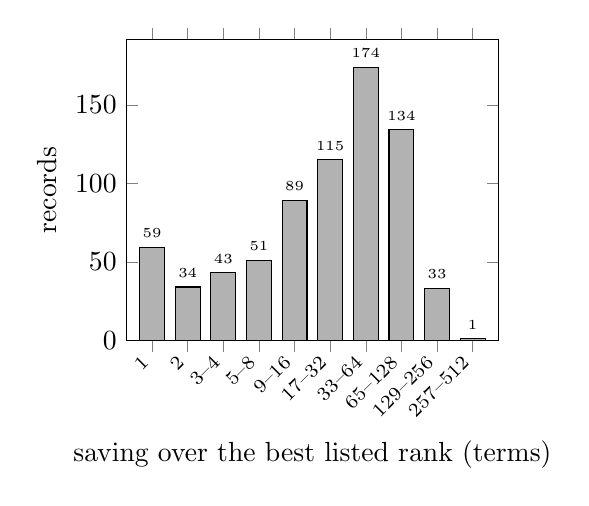
\begin{tikzpicture}
\begin{axis}[ybar,width=0.52\textwidth,height=5.4cm,bar width=9pt,ymin=0,
  symbolic x coords={1,2,3--4,5--8,9--16,17--32,33--64,65--128,129--256,257--512},xtick=data,
  xticklabel style={rotate=45,anchor=east,font=\scriptsize},xlabel={saving over the best listed rank (terms)},ylabel={records},
  nodes near coords,every node near coord/.append style={font=\tiny},enlarge x limits=0.08]
\addplot[fill=gray!60] coordinates {(1,59) (2,34) (3--4,43) (5--8,51) (9--16,89) (17--32,115) (33--64,174) (65--128,134) (129--256,33) (257--512,1)};
\end{axis}
\end{tikzpicture}\hfill
\begin{tikzpicture}
\begin{axis}[width=0.46\textwidth,height=5.4cm,xmode=log,xlabel={format volume $nmp$},ylabel={saving (\% of listed rank)},
  ymin=0,ymax=5.2,xmin=100,xmax=40000,legend style={at={(0.03,0.97)},anchor=north west,font=\scriptsize},mark size=1pt]
\addplot[only marks,mark=*,gray!75,mark options={fill=gray!60}] table[x=volume,y=relmargin] {data/scatter_nosearch.dat};
\addplot[only marks,mark=triangle*,black,mark size=1.4pt] table[x=volume,y=relmargin] {data/scatter_search.dat};
\legend{no walk or projection in the lineage,walk or projection}
\end{axis}
\end{tikzpicture}
\caption{Left: distribution of the saving over the best listed rank for the 733 records below every listed rank (octave bins). Right: relative saving against format volume for all 795 records, against the bar that defines each record's class.}
\label{fig:margins}
\end{figure}

\paragraph{The listed ranks for large formats are weak.}
92\% of the records have a side above 16, where the tables' entries are mostly not the result of a direct search but of composition over arbitrary rings (for 93.5\% of the 4{,}776 formats with a side above 16 the best rank the matmulcatalog lists is a derived entry, not an explicit scheme). A large saving against such an entry says that the entry is weak for $\F$, not that we found something hard.
The ordering of formats by saving shows it: the ten largest absolute savings (\cref{tab:top}) are all formats with a smallest side of 19 to 23 and a largest side of 27 to 32, nine of them July or committed certificates and one a projected closure product.

\section{Notable records}\label{sec:highlights}

\paragraph{Small formats.}
Only nine records have all sides at most 12 and two have all sides at most 8 (\cref{tab:small}). Of the nine, three are closure products ($\MM448$, $\MM8{8}{10}$, $\MM{10}{12}{12}$), $\MM889$ is a projection of one of them, $\MM777$ is a July construction kept by the fleet, $\MM999$ is a walk from a public scheme, and $\MM8{12}{12}$, $\MM8{11}{12}$ and $\MM7{12}{12}$ come from a chain of projected directed walks.
Neither record with all sides at most 8 is new: Table~3 of Perminov's preprint \cite{perminov2025ternary} lists rank 94 for $\MM448$ over $\mathbb Z_2$ (and 248 for $\MM777$), and \cite{medley2026gpu} reports 245 for $\MM777$.
The prior-art check of \cref{sec:persistence} leaves three of the nine: five are matched by elementary compositions of published schemes ($\MM448$, $\MM889$, $\MM8{8}{10}$, $\MM8{12}{12}$, $\MM{10}{12}{12}$), $\MM777$ is superseded, and only $\MM999$, $\MM7{12}{12}$ and $\MM8{11}{12}$ remain.
The interest of the list is what it does not contain:
$\MM444$ at rank 47 (an AlphaTensor scheme) ties and is not a record, and the best known $\MM555$ (93) and $\MM666$ (153) \cite{moosbauer2025flip} are at the tables' ranks.
\begin{table}[t]
\centering\small
\begin{tabular}{@{}lrrrp{2.7cm}l>{\raggedright\arraybackslash}p{3.5cm}@{}}
\toprule
format & rank & any ring & GF(2)-valid & class & family & note\\
\midrule
$4\times4\times8$ & 94 & 95 & 96 & \textsf{below\_all} & C & matched: $47+47$; rank 94 also in \cite{perminov2025ternary}\\
$7\times7\times7$ & 247 & 249 & 250 & \textsf{below\_all} & F & superseded: 245 reported \cite{medley2026gpu}\\
$8\times8\times9$ & 381 & 388 & 391 & \textsf{below\_all} & CP & projected closure product; matched\\
$8\times8\times10$ & 420 & 427 & 427 & \textsf{below\_all} & C & matched: $7\cdot60$\\
$9\times9\times9$ & 482 & 486 & 486 & \textsf{below\_all} & S & walk from a public scheme; also reached by the fleet; remains\\
$7\times12\times12$ & 663 & 660 & 669 & \textsf{gf2\_valid\_only} & KP & projection of the $8\times12\times12$ certificate; rational 660 listed; remains\\
$8\times11\times12$ & 673 & 676 & 690 & \textsf{below\_all} & KP & projection of the $8\times12\times12$ certificate; remains\\
$8\times12\times12$ & 705 & 720 & 735 & \textsf{below\_all} & K & directed-walk chain from $\langle8,12,15\rangle$; matched: $15\cdot47$\\
$10\times12\times12$ & 900 & 900 & 902 & \textsf{gf2\_valid\_only} & C & matched: $15\cdot60$; ties the any-ring rank\\
\bottomrule
\end{tabular}
\caption{The nine records with all sides at most 12; ``any ring'' and ``GF(2)-valid'' are the best listed ranks. For $\MM777$, Perminov's preprint \cite{perminov2025ternary} reports 248 and the Lille digest lists 249, so 247 was 2 terms below the tables' best rank (3 below their GF(2)-valid rank) and 1 below Perminov's $\mathbb Z_2$ rank; \cite{medley2026gpu} reports 245 (\cref{sec:persistence}).}
\label{tab:small}
\end{table}

\paragraph{Formats searched directly.}
Six records came from short walks (40M to 200M proposals) starting from a public integer or ternary scheme reduced modulo two: $\MM999$ (482 from Perminov's 486), $\MM{10}{13}{14}$ (1{,}150 from 1{,}152), $\MM{11}{13}{15}$ (1{,}363 from fmm-schemes' 1{,}364), $\MM{11}{14}{14}$ (1{,}372 from 1{,}373),
$\MM9{11}{13}$ (836 from 840; a rational scheme of rank 835 is listed, so this is a \textsf{gf2\_valid\_only} record) and $\MM9{10}{14}$ (819 from 820, against a listed rational 808). The savings are one to four terms.
These six are the records closest to what flip-graph searches usually report: each is the result of one walk from a public scheme, and their ranks span 482 to 1{,}372.
Of the ten formats of our first-day bundle, four were lowered or tied within two days by a new release of a public table ($\MM{13}{14}{16}$ and $\MM9{14}{16}$ lowered, $\MM8{11}{16}$ and $\MM{11}{15}{15}$ tied); three of the ten were later lowered much further by other lineages
($\MM8{11}{16}$ to 889, $\MM{13}{14}{16}$ to 1{,}763 and $\MM{11}{16}{16}$ to 1{,}707); and two, $\MM{11}{15}{15}$ and $\MM9{14}{16}$, are no longer records.

\paragraph{Squares.}
Of the five square formats among the records, $\MM777$ (247) and $\MM{13}{13}{13}$ (1{,}402, a July composition) were not found by walks; $\MM999$ (482) is a walk from a public scheme, also reached by the live fleet's walker from the same scheme; $\MM{15}{15}{15}$ (2{,}006) is a reduction, by the project's live fleet (mostly flip walkers, lane not recorded), of a July composition of rank 2{,}008; and $\MM{20}{20}{20}$ (4{,}451) is a projected July certificate. The $\MM{13}{13}{13}$, $\MM{15}{15}{15}$ and $\MM{20}{20}{20}$ records are \textsf{gf2\_valid\_only}: lower ranks (1{,}379, 1{,}977 and 3{,}995) are listed for other or unspecified rings. After the prior-art check of \cref{sec:persistence}, $\MM777$ (245 published) and $\MM{20}{20}{20}$ (4{,}371, the product of the rank-47 and a rank-93 scheme) are superseded; the other three remain.

\paragraph{Largest savings.}
\Cref{tab:top} lists the ten records with the largest absolute and relative savings over the best listed rank. All twenty have a side of at least 11 and rank in the thousands; eighteen are July or committed certificates (families J and K), one is a projected closure product and one a projected and walked one. The largest absolute saving is 268 terms for $\MM{20}{23}{32}$; the largest relative saving is 4.78\% for $\MM{15}{16}{17}$.
\begin{table}[t]
\centering\footnotesize
\begin{tabular}{@{}lrrrrl@{\hspace{7mm}}lrrrrl@{}}
\toprule
\multicolumn{6}{c}{largest absolute saving} & \multicolumn{6}{c}{largest relative saving}\\
format & rank & listed & terms & \% & fam. & format & rank & listed & terms & \% & fam.\\
\midrule
$20{\times}23{\times}32$ & 7{,}772 & 8{,}040 & 268 & 3.33 & K & $15{\times}16{\times}17$ & 2{,}329 & 2{,}446 & 117 & 4.78 & J\\
$20{\times}24{\times}31$ & 7{,}827 & 8{,}070 & 243 & 3.01 & K & $13{\times}16{\times}16$ & 1{,}930 & 2{,}022 & 92 & 4.55 & J\\
$20{\times}23{\times}28$ & 6{,}863 & 7{,}100 & 237 & 3.34 & K & $15{\times}16{\times}20$ & 2{,}716 & 2{,}834 & 118 & 4.16 & J\\
$20{\times}25{\times}31$ & 8{,}342 & 8{,}570 & 228 & 2.66 & J & $14{\times}16{\times}16$ & 2{,}041 & 2{,}128 & 87 & 4.09 & J\\
$20{\times}25{\times}27$ & 7{,}282 & 7{,}509 & 227 & 3.02 & K & $13{\times}16{\times}20$ & 2{,}417 & 2{,}516 & 99 & 3.93 & J\\
$20{\times}23{\times}31$ & 7{,}636 & 7{,}862 & 226 & 2.87 & K & $15{\times}16{\times}16$ & 2{,}137 & 2{,}223 & 86 & 3.87 & J\\
$19{\times}28{\times}28$ & 8{,}010 & 8{,}231 & 221 & 2.68 & CP & $11{\times}20{\times}28$ & 3{,}521 & 3{,}655 & 134 & 3.67 & J\\
$20{\times}23{\times}27$ & 6{,}724 & 6{,}943 & 219 & 3.15 & K & $14{\times}16{\times}17$ & 2{,}223 & 2{,}306 & 83 & 3.60 & J\\
$23{\times}32{\times}32$ & 12{,}214 & 12{,}432 & 218 & 1.75 & J & $11{\times}20{\times}32$ & 4{,}012 & 4{,}160 & 148 & 3.56 & CPW\\
$20{\times}23{\times}30$ & 7{,}427 & 7{,}638 & 211 & 2.76 & K & $13{\times}16{\times}19$ & 2{,}329 & 2{,}414 & 85 & 3.52 & J\\
\bottomrule
\end{tabular}
\caption{The ten largest absolute and relative savings among the 733 records below every listed rank. ``listed'' is the best listed rank in any ring.}
\label{tab:top}
\end{table}
Among the new records below every listed rank, the largest savings are $\MM{24}{31}{32}$ at 12{,}297 (listed 12{,}435; $-138$), $\MM{16}{20}{23}$ at 4{,}132 (4{,}260) and $\MM{16}{23}{28}$ at 5{,}656 (5{,}784).

\paragraph{Normalized exponent.}
The normalized exponent $\omega=3\ln r/\ln(nmp)$ of a scheme of rank $r$ for $\MM nmp$ is the exponent of the recursive algorithm obtained by using the scheme as its base case.
Among the records the smallest is $2.7870$ for $\MM{15}{16}{16}$ at rank 2{,}137 (the listed rank 2{,}223 gives $2.8013$); 43 records are below 2.80 (15 of them remain after the prior-art check of \cref{sec:persistence}) and none below 2.78; the median is 2.8131. For comparison the rank-47 scheme for $\MM444$ gives 2.7773 and Strassen's 2.8074.
These numbers say nothing about the asymptotic exponent of matrix multiplication, which is far below them \cite{alman2025asymmetry,dupont2026omega}; they matter only for recursive algorithms over $\F$ with small base cases.

\section{What the records are compared with}\label{sec:comparators}

A record is a statement about a bar. The choice and reading of the bars determine how much it means, so we report them in detail.

\paragraph{Which table sets the bar.}
For each record we re-derived the bar from the four tables at the pinned revisions (all 795 agree with the archive's index). \Cref{tab:suppliers} shows which sources attain the any-ring bar. The matmulcatalog attains it for 707 of the 795 records and is the only source at that rank for 273; the Lille digest attains it for 519 and alone for 86; FastMatrixMultiplication attains it for 46 and never alone (through a rational scheme in 33 cases, a ternary one in 13 and an integer one in 3; a record can tie several rings); fmm-schemes attains it for two records, alone in both.
\begin{table}[t]
\centering\small
\begin{tabular}{@{}lrrrr@{}}
\toprule
records attaining the any-ring bar through & Lille & matmulcatalog & FMM & fmm-schemes\\
\midrule
\textsf{below\_all} (733): attain (sole) & 465 (70) & 661 (265) & 31 (0) & 2 (2)\\
\textsf{gf2\_valid\_only} (62): attain (sole) & 54 (16) & 46 (8) & 15 (0) & 0 (0)\\
all 795: attain (sole) & 519 (86) & 707 (273) & 46 (0) & 2 (2)\\
\bottomrule
\end{tabular}
\caption{Which table supplies the best listed rank in any ring (ties counted for every attaining source; ``sole'' = the only source at that rank). FMM by ring: Q 33, ZT 13, Z 3 (a record may tie with several).}
\label{tab:suppliers}
\end{table}

\paragraph{No GF(2)-valid bar for 458 of the 733 strongest records.}
The Lille digest, which sets the any-ring bar alone or jointly for 465 of the 733 \textsf{below\_all} records, records no field, so its rank may or may not be achievable over $\F$. For 458 of the 733 records no scheme known to be valid over $\F$ is listed at all: the any-ring bar (matmulcatalog for 403 of them, Lille for 291, with ties counted) is the only bar.
For the other 275 the GF(2)-valid bar is defined and we are below it by a median of 19 terms (0.95\%, maximum 268). The two readings answer different questions: ``below every listed rank'' says that no listed scheme, over any ring, is as small; it does not say that a scheme of that size was not already known over $\F$ (for example in a paper), only that it is not in the tables.
Conversely, where no GF(2)-valid scheme is listed at all (1{,}025 formats classed \textsf{above} and 68 classed \textsf{tie}), a scheme of ours that lies at or above a listed rank of unspecified field (Lille) or of another field (matmulcatalog) is not a record, although it may be the best scheme known over $\F$; the records therefore undercount the formats for which we hold the best known scheme over $\F$.

\paragraph{The 62 \textsf{gf2\_valid\_only} records.}
For 55 of them the Lille digest lists a rank at or below ours (field unspecified), for the other seven only a matmulcatalog scheme over another field does. For 17 of the 62 a rational scheme of the FastMatrixMultiplication repository is at or below our rank (15 in its rational directory and 2 in its \texttt{known} directory, for $\MM{13}{13}{13}$ and $\MM{15}{15}{15}$); all 17 have an even denominator, so none reduces modulo two.
Twenty of the 298 rational files use only odd denominators and do reduce to exact schemes over $\F$; none of them is below our scheme for its format.

\paragraph{Commutative algorithms are excluded.}
The matmulcatalog also lists commutative algorithms (Waksman's rank 473 for $\MM999$, for instance) \cite{waksman1970winograd,winograd1968inner}. These are not decompositions of the tensor and do not bound its rank; they cannot be composed recursively into matrix algorithms. We exclude them. The catalogue does not stamp them F2, so counting them in the any-ring bar alone would move $\MM777$ and $\MM999$ from \textsf{below\_all} to \textsf{gf2\_valid\_only}; but a commutative entry lies at or below our rank for five records, and all five would be lost if commutative algorithms were also counted as valid over $\F$:
\begin{center}\small
\begin{tabular}{@{}lrr@{}}
\toprule
format & our rank & commutative entry\\\midrule
$7\times7\times7$ & 247 & 235\\
$9\times9\times9$ & 482 & 473\\
$13\times13\times13$ & 1{,}402 & 1{,}333\\
$15\times15\times15$ & 2{,}006 & 2{,}003\\
$20\times20\times20$ & 4{,}451 & 4{,}390\\
\bottomrule
\end{tabular}
\end{center}

\paragraph{The catalogue's F2 stamp over-claims.}
Derived entries stamped F2 in the matmulcatalog may need a leaf that is valid over another field only (for $\MM336$ the best rank is 40 for $\mathbb F_3$, $\mathbb Q$, $\mathbb R$ and $\mathbb C$ but 42 with an F2 stamp; for $\MM338$ 55 and 56; for $\MM245$ 32 and 33).
When we replay its recipes over $\F$ (companion paper), 110 of 373 and 144 of 979 targets fail at the catalogue's rank. Its F2 minima can therefore be lower than what is achievable over $\F$, which makes the \textsf{gf2\_valid\_only} comparison conservative.

\section{Persistence: re-scoring and prior art}\label{sec:persistence}

\paragraph{Re-scoring against later revisions.}
The four tables kept changing on the day of scoring and after it (\cref{tab:rescore}). We therefore re-scored all 795 records against the revisions current at 21:33 UTC on 2026-09-29, about eight hours after the scoreboard of \cref{sec:overview}.
The scoring rule applied to the pinned inputs reproduces the bars and the class of every record, and the same tables rebuilt from fresh clones at the pinned revisions are identical; applied to the later revisions the rule leaves 793 records unchanged and lowers two margins, both because the Lille digest gained a lower rank:
$\MM{11}{11}{17}$ (ours 1{,}312; the listed rank fell from 1{,}314 to 1{,}313, so the margin is now one term) and $\MM{16}{16}{31}$ (ours 4{,}346; 4{,}474 fell to 4{,}460, a margin of 114 terms instead of 128).
No record changed class and none was lost. The four heads had not moved when we checked again two hours later, but a re-scoring on the day of submission will still be needed.
\begin{table}[t]
\centering\small
\begin{tabular}{@{}lll@{}}
\toprule
source & pinned at scoring (2026-09-29) & latest (2026-09-29, 21:33 UTC)\\
\midrule
Lille digest & \texttt{9f26324} & \texttt{f5c2b26}\\
matmulcatalog & \texttt{f0c2ba9} & \texttt{5a30652}\\
FastMatrixMultiplication & \texttt{613599b} & \texttt{ac13ca8}\\
fmm-schemes & \texttt{8fa0f2a} & \texttt{8fa0f2a} (unchanged)\\
\bottomrule
\end{tabular}
\caption{Revisions of the four tables at scoring and at the re-scoring.}
\label{tab:rescore}
\end{table}

\paragraph{What the scoring rule does not read.}
The four tables are not a complete record of GF(2)-valid prior art. The scoring rule reads the schemes of the catalogue file \texttt{catalog.json}, the ranks of the Lille digest and the ranks and rings encoded in the file names of the scheme files of the two repositories. It does not read
(i) schemes valid only in characteristic two that are published outside the tables: Arai et al.'s $\MM455$ of rank 73 \cite{arai2024adaptive}, Kauers and Wood's $\MM456$ of rank 89 over $\mathbb Z_2$ \cite{kauers2025meta}, Medley et al.'s $\MM777$ of rank 245 \cite{medley2026gpu} and the $\mathbb Z_2$ discoveries of Perminov's Table~3 \cite{perminov2025ternary};
(ii) the rank claims that the matmulcatalog keeps without factor matrices in its file \texttt{docs/cited-bounds.json}, which has 6{,}524 entries, was public in the revision we scored, and includes 971 serendipitous-product claims of Perminov \cite{perminov2026serendipitous} for formats with largest side 18 to 32;
(iii) compositions (direct sums, Kronecker products, Strassen's algorithm on unequal blocks) of the schemes that the tables do list.

\paragraph{The prior-art check.}
On the evening of 2026-09-29 we read the result tables of 48 arXiv papers (one turned out to be unrelated) and the README of one repository: 770 rows of Perminov's three rank papers were parsed from the text (each table's row count equals the count the paper states) and 878 rows of 34 further sources were transcribed with their line and a verbatim quote, each re-checked mechanically against the text. A row counts as valid over $\F$ only if the source states characteristic two, $\mathbb Z_2$, ternary or integer coefficients, or an arbitrary ring; a field that is not stated is never counted.
We then computed the smallest rank reachable from listed and published GF(2)-valid ranks by direct sums, Kronecker products and Strassen's algorithm on unequal blocks; built every composition of explicit published scheme files whose rank is at or below one of ours (146 schemes) and rebuilt the catalogue's serendipitous-product claims from the FastMatrixMultiplication base schemes named there, reduced modulo two; and verified every scheme exactly over $\F$ with a numpy-based check. Nine of these schemes (eight that supersede ours and one that matches it) were also verified with the verifier of our release, and an independent re-check of all 185 schemes that we rebuilt, with two further implementations, agreed.

\begin{table}[t]
\centering\small
\begin{tabular}{@{}lrrr@{}}
\toprule
prior art found & records & \textsf{below\_all} & \textsf{gf2\_valid\_only}\\
\midrule
superseded: a scheme built from published files, verified & 80 & 65 & 15\\
superseded: a published rank claim, not reproduced by us & 7 & 6 & 1\\
matched: a composition of published schemes, built and verified & 105 & 88 & 17\\
matched: a published rank claim & 7 & 5 & 2\\
\textsf{below\_all} contradicted only by a rational claim & 9 & 9 & --\\
none found & 587 & 560 & 27\\
\midrule
all & 795 & 733 & 62\\
\bottomrule
\end{tabular}
\caption{Outcome of the prior-art check; each record has the first flag that applies, in the order of the rows.}
\label{tab:priorart}
\end{table}

\paragraph{Outcome.}
For 80 records we built, from published material, a scheme over $\F$ of smaller rank than ours, and every one verifies exactly (\cref{tab:priorart}). Of these, 43 are serendipitous products whose rank claims the matmulcatalog has carried since 2026-06-16, 36 are compositions of explicit published schemes and one is Medley et al.'s $\MM777$ of rank 245.
The ingredients of the compositions are most often schemes valid only in characteristic two that the four tables lack, above all Arai et al.'s $\MM455$ of rank 73 (30 of the 36), together with AlphaTensor's rank-47 scheme for $\MM444$ and Perminov's ternary schemes. For example, the Kronecker product of the rank-47 scheme for $\MM444$ and a rank-93 scheme for $\MM555$ \cite{moosbauer2025flip} has rank 4{,}371 and supersedes our $\MM{20}{20}{20}$ at 4{,}451.
For seven more records a published rank claim lies below ours. For four of these we tried to rebuild the claim from the base schemes it names and did not reach it (the $\MM{9}{9}{18}$ claim fits only a rational scheme), and the other three, like the seven matches by claim below, compose listed ranks that include catalogue-derived entries, which carry the caveat of the F2 stamp (\cref{sec:comparators}). \emph{We withdraw all 87 records}, which is the conservative choice.
For 112 further records our rank equals that of a composition of published schemes (105 built and verified, of which 102 are compositions and three serendipitous products; seven by claim); these are composition bounds and not search results, and most of them (96 of the 112) are closure products of our own.
For nine \textsf{below\_all} records the matmulcatalog records a lower rank over the rationals (sixteen records carry such a claim, seven of them also flagged above), so that the label ``below every listed rank in any ring'' is contradicted while the GF(2) comparison stands.
That leaves \textbf{596 records} (587 with no prior art found, and those nine) that remain below every GF(2)-valid bound we could find or build.

\begin{table}[t]
\centering\small
\begin{tabular}{@{}p{7.2cm}lrrrr@{}}\toprule
lineage of the recorded tensor & code & records & superseded & matched & remaining\\\midrule
closure product (block sums and Kronecker products of exact schemes) & C & 203 & 32 & 96 & 75\\
July 2026 block-composition certificate & J & 152 & 6 & 7 & 139\\
certificate committed 2026-09-22 to 09-26 & K & 126 & 7 & 3 & 116\\
closure product, projected and walked (in several rounds) & CPW & 106 & 11 & 1 & 94\\
replayed recipe, then walked & MW & 58 & 9 & 1 & 48\\
July certificate, projected & JP & 36 & 3 & 0 & 33\\
matmulcatalog recipe replayed over $\F$ & M & 24 & 10 & 2 & 12\\
committed certificate, projected and walked & KPW & 23 & 3 & 0 & 20\\
July certificate, projected and walked & JPW & 15 & 3 & 0 & 12\\
closure product, then projected & CP & 15 & 0 & 2 & 13\\
replayed recipe, projected and walked & MPW & 12 & 2 & 0 & 10\\
closure product, then walked & CW & 8 & 0 & 0 & 8\\
committed certificate, projected & KP & 8 & 0 & 0 & 8\\
public integer scheme reduced mod 2, then walked & S & 6 & 0 & 0 & 6\\
live-fleet construction/checkpoint & F & 2 & 1 & 0 & 1\\
replayed recipe, then projected & MP & 1 & 0 & 0 & 1\\
\midrule
all & & 795 & 87 & 112 & 596\\
\bottomrule\end{tabular}

\caption{Prior-art outcome by lineage family (codes as in \cref{tab:families}). ``Superseded'' and ``matched'' are as in \cref{tab:priorart}; ``remaining'' includes the nine rational-claim cases.}
\label{tab:priorart-family}
\end{table}

\paragraph{Where the prior art bites.}
The check hits the closure products hardest (128 of 203 are superseded or matched; \cref{tab:priorart-family}), as one expects of compositions: the tables did not compose everything they could. The block recombinations of July and the certificates descended from them mostly remain (13 of 152 July certificates and 10 of 126 committed certificates are flagged), and so do the records that come from walks (35 of the 288 with a walk or a projection in their lineage are flagged).
By size, none of the two records with all sides at most 8 remains and three of the seven with largest side 9 to 12 do; 41 of the 52 with largest side 13 to 16 and 552 of the 734 above 16 remain.
The ten largest absolute and the ten largest relative savings (\cref{tab:top}), and the record with the best normalized exponent ($\MM{15}{16}{16}$), all remain. The median saving of the 596 is 29 terms (0.92\%).

\paragraph{Composing everything public.}
The check asks whether our records are beaten. The converse question is what a closure over every public GF(2)-valid scheme would give for all 5{,}456 formats. A rank-only estimate, by direct sums, Kronecker products and Strassen's algorithm on unequal blocks, from the ranks of the four tables puts 276 formats below the tables, 52 of them not among our 795, because the tables are not closed under composition. Adding the published GF(2)-valid ranks above (some of them claims for which we hold no scheme) gives 461 formats, 174 of them not among our 795, and adding our own witnesses gives 984, that is 189 more than our 795, and lowers 56 of the 795 (median 18.5 terms).
We did not build these schemes. The estimate leaves out serendipitous products, the July block recombination with the newer leaves, projection and walks, so it is a lower bound on what a full run over the union of the public schemes would give. It makes the same point as the check: against tables that are not closed under composition, ``below the tables'' is a weak claim of novelty.

\paragraph{Direct overlaps with the literature.}
Two of our shapes appear in a published table at or below our rank. Medley et al.\ \cite{medley2026gpu} report $\MM777$ over $\F$ with 245 multiplications, below our 247; we decoded the scheme printed in their appendix and verified it. Perminov's Table~3 \cite{perminov2025ternary}, which lists 30 improvements over $\mathbb Z_2$, has $\MM448$ at rank 94, equal to ours (and to $47+47$); it also has $\MM777$ at 248.
No other table we read states a rank valid over $\F$ at or below ours for one of our shapes; lower ranks over the rationals, or with no stated field, exist for some (see above and \cref{sec:comparators}). The prior art that matters is in compositions and in one catalogue file, not in direct searches of these formats.

\paragraph{What the check does not cover.}
The check is limited. It reads 48 arXiv papers found by searching and by following references on one evening; it builds compositions only from explicit published scheme files; it uses a paper's rank only where the paper states the field; and it knows four constructions (direct sums, Kronecker products, Strassen's algorithm on unequal blocks, serendipitous products). A source we did not find, a scheme that exists only as an unpublished claim, or another construction could supersede more records. ``None found'' means no more than that, and the 596 are not optimality claims.
The other sections describe all 795 records, because the scoring rule did not see this prior art; \cref{app:all} marks the status of every record, and the statements that change for the 596 are given in this section.

\section{Verification and provenance}\label{sec:verification}

\paragraph{Exactness.}
A record is a list of triples of bit vectors whose sum is the matrix-multiplication tensor (\cref{sec:setting}). Each of the 795 records was checked by two separately written implementations: a sparse cancellation count in Python and a dense comparison with the closed form in Ruby; the native walker checks a third time the input and output of every walk. Both checkers reject a single flipped bit, a dropped term and an output factor in the transposed layout of the public files (the negative controls are in the companion paper).
The Ruby check ran on the 691 records held in the release bundles and on the 661 chain heads of the bundles (logs in the release), and later on all 1{,}089 tensors behind the records: the 985 distinct tensors of the bundles, the 102 committed certificates that stay in the repository and the two fleet checkpoints (log in the repository); every one is exact at the rank of its manifest or index row, and every bundle file has the hash of its manifest row. The verification runs of the release itself (A--D) used the Python gate only.
Both checkers were written by the same author and share the bit layout, which is the weakest point of this claim.

\paragraph{Identity and lineage.}
A tensor is identified by the SHA-256 of its canonical text (sorted, duplicate-free triples). The index gives, for every record, the format, the rank, the best listed rank in any ring and among GF(2)-valid schemes, the two margins, the class, the lineage family, the SHA-256 and the holding asset. Each record ends a chain of rows, from a seed (a public scheme reduced modulo two, a replayed catalogue recipe, a closure recipe or a committed certificate) through projections, basis rewrites and walks, in one of four bundles.
The verifier re-derived from pinned upstream files or from git history all 11 distinct public seeds, all 186 archived July certificates, matched the 25 retained committed certificates against the repository files, recomputed all 225 projection rows and reproduced 71 of the 82 catalogue replays from an empty cache; and it replayed 42 of the 244 distinct walks byte for byte with the native walker. The other walks were checked for exactness and for the invariant that a walk keeps the format and never raises the rank.
Running the shipped verifier on the extracted release reproduces its five logs exactly.

\paragraph{What is not established.}
Five replayed seeds, and the eight records that depend on them, were built from two local leaves (schemes for $\MM448$ and $\MM{12}{15}{16}$) that their manifest does not list: the tensors are exact, but their leaf provenance is incomplete, and the archive's description of them as ``equal-rank variants'' of an empty-cache replay is wrong (they are lower-rank first-pass constructions).
A separate script rebuilt 259 of the 267 closure rows byte for byte; the other eight rows, six distinct records, depend on three intermediate witnesses whose files no longer exist, and 43 of 1{,}098 replays give a tensor of the same rank that differs from what an empty cache gives, through a cache-order defect that is fixed and described in the companion paper. None of this affects exactness or rank.
The record index also carries two wrong lineage labels, corrected in this paper: it lists $\MM999$ and $\MM{13}{13}{13}$ under ``live fleet checkpoint'', whereas the first is a walk from a public scheme and the second the July certificate itself.
The steps by which the 126 committed certificates were produced before the campaign are documented in the repository's certificate directories, and were not replayed for this release.

\section{Limitations, claim status and availability}\label{sec:limits}

\paragraph{What the records are.}
Each record is an exact upper bound on the rank of $\MM nmp$ over $\F$, and nothing more: not a lower bound, not an optimality claim, and not a statement about any other ring. The schemes rely on characteristic two (the rank-47 scheme for $\MM444$ in particular) and are not known to lift to the integers or the rationals (no lift was attempted); they must not be advertised as records for those rings.
``Record'' means smaller than the entries of four tables at named revisions on 2026-09-29. It does not mean new to the literature. Under the claim policy of the project, in which a result that improves the project's baseline but has not been searched against the literature is labelled \emph{apparent}, that is the label we use, and the persistence check of \cref{sec:persistence}, which supersedes 87 of the 795 and matches 112 more, is a first step towards an audit, not the audit.

\paragraph{Most of the results are consequences of known constructions.}
Composition dominates (\cref{sec:nature}), and the constructions used are established: block sums, Kronecker products, block recombination with a rank-47 outer scheme \cite{sedoglavic2017seven,drevet2011optimization}, Perminov's serendipitous product \cite{perminov2026serendipitous}, coordinate projection. What is new is the application of these constructions to the schemes that are best in characteristic two, at a scale (the 5{,}456 formats up to $32\times32\times32$) that the tables did not cover over $\F$, and the exact record of each derivation. A lower rank for one leaf changes many records at once, so the list should be read as a snapshot of a compositional frontier, not as 795 independent discoveries; the prior-art check makes the point, since 199 of the 795 are superseded or matched by compositions and claims built from published schemes.

\paragraph{Comparators.}
The tables are moving, incomplete and of mixed field (\cref{sec:comparators}), and they omit GF(2)-valid prior art that is public (\cref{sec:persistence}). For 458 of the 733 strongest records no GF(2)-valid scheme is listed, so the bar is a rank whose field is unknown; conversely, where no GF(2)-valid scheme is listed, a scheme of ours above the listed rank is not a record even if it is the best known over $\F$, so the list undercounts. The scoring rules exclude commutative algorithms and never count a rational scheme as valid over $\F$; twenty of the 298 rational files have only odd denominators and would reduce modulo two, but none is below our rank for its format.
The records come from a single scoreboard at a single date; a re-scoring at a later date can lower or remove entries, as the July certificates show (23 of the 186 were no longer records by late September).

\paragraph{Coverage and search depth.}
We hold a verified scheme for 3{,}662 of the 5{,}456 formats (67.1\%): for every format with largest side at most 16, for 70\% of those with largest side 17--24 and for 59\% of those with 25--32. That a format is not a record says little about the tables' rank for it. The search was finite (about $3\times10^{11}$ walk proposals in the campaign, not counting the earlier stages and the fleet; \cite{peterson2026methods}); we make no claim that any rank is a local or global minimum of the search space, and we did not attempt formats with a side above 32.

\paragraph{Verification.}
Exactness is established directly, twice, by code from one author with a shared bit layout. The provenance is re-derived only in part (\cref{sec:verification}): 42 of 244 walks were replayed, five seeds and eight records have incomplete leaf provenance, and the steps of the committed certificates are documented but were not replayed.

\paragraph{Attribution and licensing.}
Every derived tensor keeps the credit of the schemes it starts from, recorded per row: Perminov's FastMatrixMultiplication (MIT), Witteveen's fmm-schemes (CC BY 4.0), the matmulcatalog of Lacelle, which carries no licence file, and the Lille catalogue of Sedoglavic, used for comparison only.
The project owner treats decompositions as mathematical objects that are redistributed with attribution; \todo{confirm with the matmulcatalog authors before publication, as their repository has no licence}.

\paragraph{Availability.}
The search and verification tools are in the package \texttt{tungsten-metaflip} (SPDX: MIT OR Apache-2.0 WITH LLVM-exception) of the Tungsten repository \cite{tungsten2026lang}, branch \texttt{metaflip-\allowbreak public-\allowbreak ternary-\allowbreak gf2} (the tools of the release are commit \texttt{00ffa04f9}; the sources of these papers, their scripts and the verification logs are in later commits of the branch) \todo{push and merge the branch before submission}.
The lineage bundles (which hold 691 of the 795 record tensors with their derivations), the record index with the best listed ranks and margins, the fleet checkpoints, the verification logs and a snapshot of the tools are release \texttt{evidence-2026-09-29} of \texttt{tungsten-lang/metaflip-archives}, currently private \todo{deposit publicly, for example on Zenodo, and cite the DOI}; the other 102 records are committed certificates of the repository, and the logs of the later Ruby check and of the closure rebuild are in the repository as well (\texttt{papers/verification}). The scripts of the prior-art check, the transcribed literature rows with their quotes, the per-record flags and the 185 schemes we rebuilt are described in \texttt{papers/prior-art} of the repository \todo{deposit the rebuilt schemes and the fetched texts with the release}. Appendix~\ref{app:all} lists every record with its format, rank, bars, class and lineage family.


\section*{Acknowledgements and disclosure}
The search campaign, the tooling and the drafting of this manuscript were assisted by Claude (Anthropic); the author is responsible for the content.
The results build on the schemes and tables of many authors (Hopcroft and Kerr, Sedoglavic, Fawzi et al., Kauers and Moosbauer, Arai et al., Moosbauer and Poole, Kauers and Wood, Medley et al., Perminov, Witteveen, Lacelle and others cited in the text); every derived tensor keeps their credit, recorded per row in the data release.
\todo{funding / conflicts-of-interest statement}

\bibliographystyle{plainnat}
\bibliography{refs}

\appendix
\section{Family codes}\label{app:families}
\begin{tabular}{@{}llr@{}}\toprule code & lineage of the recorded tensor & records\\\midrule
C & closure product (block sums and Kronecker products of exact schemes) & 203\\
J & July 2026 block-composition certificate & 152\\
K & certificate committed 2026-09-22 to 09-26 & 126\\
CPW & closure product, projected and walked (in several rounds) & 106\\
MW & replayed recipe, then walked & 58\\
JP & July certificate, projected & 36\\
M & matmulcatalog recipe replayed over $\F$ & 24\\
KPW & committed certificate, projected and walked & 23\\
JPW & July certificate, projected and walked & 15\\
CP & closure product, then projected & 15\\
MPW & replayed recipe, projected and walked & 12\\
CW & closure product, then walked & 8\\
KP & committed certificate, projected & 8\\
S & public integer scheme reduced mod 2, then walked & 6\\
F & live-fleet construction/checkpoint & 2\\
MP & replayed recipe, then projected & 1\\
\bottomrule\end{tabular}


\section{All 795 records}\label{app:all}
\begingroup\scriptsize\setlength{\tabcolsep}{3.2pt}
\begin{longtable}{@{}lrrrl@{\hspace{6mm}}lrrrl@{}}
\caption{All 795 records of 2026-09-29, ordered by largest, middle and smallest side (the right column continues the left). Columns: format (sorted), our rank, best listed rank in any ring, best listed GF(2)-valid rank (-- if none), family code (Appendix~\ref{app:families}). Superscripts: $\dagger$ below the GF(2)-valid bar only; S superseded and M matched by published constructions or claims, Q a lower rational claim exists (\cref{sec:persistence}); no letter: no prior art found.}\label{tab:all}\\
\toprule format & rank & any & F$_2$ & fam. & format & rank & any & F$_2$ & fam.\\\midrule\endfirsthead
\toprule format & rank & any & F$_2$ & fam. & format & rank & any & F$_2$ & fam.\\\midrule\endhead
\bottomrule\endlastfoot
$7{\times}7{\times}7$ & 247 & 249 & 250 & F$^{\mathrm{S}}$ & $14{\times}16{\times}26$ & 3407 & 3458 & -- & K\\
$4{\times}4{\times}8$ & 94 & 95 & 96 & C$^{\mathrm{M}}$ & $15{\times}16{\times}26$ & 3608 & 3624 & -- & C$^{\mathrm{M}}$\\
$8{\times}8{\times}9$ & 381 & 388 & 391 & CP$^{\mathrm{M}}$ & $16{\times}16{\times}26$ & 3767 & 3797 & -- & C\\
$9{\times}9{\times}9$ & 482 & 486 & 486 & S & $8{\times}17{\times}26$ & 2162 & 2191 & -- & K\\
$8{\times}8{\times}10$ & 420 & 427 & 427 & C$^{\mathrm{M}}$ & $10{\times}17{\times}26$ & 2679 & 2681 & 2681 & MW\\
$8{\times}11{\times}12$ & 673 & 676 & 690 & KP & $16{\times}17{\times}26$ & 4111 & 4122 & -- & C\\
$7{\times}12{\times}12$ & 663 & 660 & 669 & KP$^{\dagger}$ & $8{\times}18{\times}26$ & 2274 & 2275 & 2275 & K\\
$8{\times}12{\times}12$ & 705 & 720 & 735 & K$^{\mathrm{M}}$ & $11{\times}18{\times}26$ & 3088 & 3092 & 3092 & MW\\
$10{\times}12{\times}12$ & 900 & 900 & 902 & C$^{\dagger\mathrm{M}}$ & $7{\times}19{\times}26$ & 2209 & 2215 & -- & K\\
$9{\times}11{\times}13$ & 836 & 835 & 840 & S$^{\dagger}$ & $8{\times}19{\times}26$ & 2366 & 2419 & 2419 & K\\
$8{\times}12{\times}13$ & 786 & 781 & 807 & K$^{\dagger}$ & $11{\times}19{\times}26$ & 3279 & 3280 & -- & JPW\\
$12{\times}13{\times}13$ & 1292 & 1274 & 1298 & JP$^{\dagger}$ & $12{\times}19{\times}26$ & 3461 & 3475 & -- & C\\
$13{\times}13{\times}13$ & 1402 & 1379 & 1426 & J$^{\dagger}$ & $13{\times}19{\times}26$ & 3761 & 3835 & -- & K\\
$4{\times}4{\times}14$ & 162 & 163 & 164 & C$^{\mathrm{M}}$ & $16{\times}19{\times}26$ & 4541 & 4568 & -- & KP\\
$4{\times}5{\times}14$ & 206 & 206 & 207 & C$^{\dagger\mathrm{S}}$ & $7{\times}20{\times}26$ & 2279 & 2300 & 2300 & C\\
$9{\times}10{\times}14$ & 819 & 808 & 820 & S$^{\dagger}$ & $8{\times}20{\times}26$ & 2459 & 2506 & -- & C$^{\mathrm{M}}$\\
$8{\times}12{\times}14$ & 849 & 843 & 861 & K$^{\dagger}$ & $11{\times}20{\times}26$ & 3329 & 3428 & 3428 & J\\
$12{\times}12{\times}14$ & 1251 & 1232 & 1260 & J$^{\dagger}$ & $12{\times}20{\times}26$ & 3566 & 3624 & -- & C$^{\mathrm{M}}$\\
$10{\times}13{\times}14$ & 1150 & 1152 & 1152 & S & $13{\times}20{\times}26$ & 3984 & 4002 & -- & K\\
$12{\times}13{\times}14$ & 1383 & 1370 & 1389 & JP$^{\dagger}$ & $16{\times}20{\times}26$ & 4634 & 4776 & -- & K$^{\mathrm{M}}$\\
$13{\times}13{\times}14$ & 1501 & 1511 & 1511 & J & $11{\times}21{\times}26$ & 3615 & 3628 & -- & C\\
$11{\times}14{\times}14$ & 1372 & 1373 & 1373 & S & $16{\times}21{\times}26$ & 4908 & 4969 & -- & K\\
$4{\times}4{\times}15$ & 175 & 176 & 176 & C$^{\mathrm{M}}$ & $11{\times}22{\times}26$ & 3771 & 3776 & -- & C\\
$4{\times}5{\times}15$ & 220 & 221 & 221 & C$^{\mathrm{S}}$ & $15{\times}22{\times}26$ & 4936 & 4966 & -- & K\\
$8{\times}8{\times}15$ & 632 & 628 & 639 & CPW$^{\dagger\mathrm{S}}$ & $16{\times}22{\times}26$ & 5136 & 5182 & -- & K\\
$8{\times}12{\times}15$ & 899 & 904 & 914 & K & $20{\times}22{\times}26$ & 6340 & 6277 & 6448 & JPW$^{\dagger}$\\
$12{\times}12{\times}15$ & 1320 & 1280 & 1326 & JP$^{\dagger}$ & $8{\times}23{\times}26$ & 2866 & 2884 & -- & CPW\\
$8{\times}13{\times}15$ & 989 & 991 & 991 & K & $15{\times}23{\times}26$ & 5129 & 5167 & -- & K\\
$11{\times}13{\times}15$ & 1363 & 1364 & 1364 & S & $20{\times}23{\times}26$ & 6508 & 6585 & -- & K\\
$12{\times}13{\times}15$ & 1455 & 1442 & 1464 & JP$^{\dagger}$ & $7{\times}24{\times}26$ & 2720 & 2727 & -- & C\\
$13{\times}13{\times}15$ & 1582 & 1605 & 1605 & J & $8{\times}24{\times}26$ & 2932 & 2936 & 2936 & C$^{\mathrm{S}}$\\
$13{\times}15{\times}15$ & 1796 & 1776 & 1797 & J$^{\dagger}$ & $10{\times}24{\times}26$ & 3696 & 3680 & 3700 & C$^{\dagger\mathrm{S}}$\\
$15{\times}15{\times}15$ & 2006 & 1977 & 2058 & F$^{\dagger}$ & $19{\times}24{\times}26$ & 6561 & 6576 & -- & KPW\\
$4{\times}5{\times}16$ & 234 & 235 & 235 & C$^{\mathrm{S}}$ & $20{\times}24{\times}26$ & 6684 & 6747 & 6906 & K\\
$8{\times}8{\times}16$ & 658 & 665 & 666 & C$^{\mathrm{M}}$ & $11{\times}25{\times}26$ & 4282 & 4283 & -- & CW\\
$8{\times}11{\times}16$ & 889 & 904 & 906 & CPW & $20{\times}25{\times}26$ & 7130 & 7167 & -- & K\\
$7{\times}12{\times}16$ & 871 & 876 & 876 & K & $20{\times}26{\times}26$ & 7370 & 7408 & 7566 & K\\
$8{\times}12{\times}16$ & 940 & 956 & 960 & C$^{\mathrm{M}}$ & $2{\times}4{\times}27$ & 172 & 172 & 176 & C$^{\dagger\mathrm{M}}$\\
$11{\times}12{\times}16$ & 1301 & 1278 & 1306 & JP$^{\dagger}$ & $4{\times}5{\times}27$ & 394 & 395 & 395 & C$^{\mathrm{S}}$\\
$12{\times}12{\times}16$ & 1363 & 1380 & 1380 & J$^{\mathrm{M}}$ & $8{\times}8{\times}27$ & 1107 & 1108 & -- & CPW$^{\mathrm{M}}$\\
$7{\times}13{\times}16$ & 962 & 962 & 966 & K$^{\dagger}$ & $11{\times}12{\times}27$ & 2163 & 2166 & -- & CPW\\
$8{\times}13{\times}16$ & 1037 & 1054 & 1064 & CP & $11{\times}13{\times}27$ & 2359 & 2393 & -- & J\\
$11{\times}13{\times}16$ & 1452 & 1446 & 1458 & JP$^{\dagger}$ & $12{\times}13{\times}27$ & 2517 & 2529 & -- & C\\
$12{\times}13{\times}16$ & 1507 & 1509 & 1544 & J & $3{\times}14{\times}27$ & 842 & 843 & 843 & C$^{\mathrm{S}}$\\
$13{\times}13{\times}16$ & 1648 & 1704 & 1711 & J & $11{\times}14{\times}27$ & 2539 & 2555 & -- & J\\
$12{\times}14{\times}16$ & 1626 & 1617 & 1663 & JP$^{\dagger}$ & $12{\times}14{\times}27$ & 2663 & 2697 & -- & K\\
$13{\times}14{\times}16$ & 1763 & 1796 & 1806 & J & $4{\times}15{\times}27$ & 1065 & 1068 & 1068 & MW$^{\mathrm{M}}$\\
$14{\times}14{\times}16$ & 1881 & 1895 & 1943 & J & $11{\times}15{\times}27$ & 2694 & 2703 & 2703 & J\\
$8{\times}15{\times}16$ & 1177 & 1185 & 1203 & CPW & $12{\times}15{\times}27$ & 2839 & 2840 & -- & KPW\\
$12{\times}15{\times}16$ & 1714 & 1725 & 1725 & J & $13{\times}15{\times}27$ & 3126 & 3155 & -- & K\\
$13{\times}15{\times}16$ & 1858 & 1885 & 1885 & J & $11{\times}16{\times}27$ & 2825 & 2847 & -- & K$^{\mathrm{S}}$\\
$14{\times}15{\times}16$ & 1975 & 2016 & 2043 & J & $12{\times}16{\times}27$ & 2957 & 2964 & -- & CPW\\
$15{\times}15{\times}16$ & 2074 & 2132 & 2132 & J & $13{\times}16{\times}27$ & 3256 & 3346 & -- & K\\
$7{\times}16{\times}16$ & 1135 & 1148 & 1158 & CPW & $16{\times}16{\times}27$ & 3904 & 3944 & -- & CPW\\
$8{\times}16{\times}16$ & 1222 & 1230 & 1256 & C$^{\mathrm{M}}$ & $8{\times}17{\times}27$ & 2247 & 2248 & -- & JP\\
$10{\times}16{\times}16$ & 1558 & 1560 & 1578 & J & $10{\times}17{\times}27$ & 2766 & 2767 & 2767 & MW\\
$11{\times}16{\times}16$ & 1707 & 1724 & 1749 & JP & $14{\times}17{\times}27$ & 3818 & 3820 & 3820 & MW\\
$12{\times}16{\times}16$ & 1786 & 1815 & 1862 & J$^{\mathrm{M}}$ & $16{\times}17{\times}27$ & 4259 & 4278 & -- & C\\
$13{\times}16{\times}16$ & 1930 & 2022 & 2038 & J & $8{\times}18{\times}27$ & 2334 & 2338 & 2338 & M$^{\mathrm{M}}$\\
$14{\times}16{\times}16$ & 2041 & 2128 & 2170 & J & $4{\times}19{\times}27$ & 1340 & 1344 & 1344 & MW\\
$15{\times}16{\times}16$ & 2137 & 2223 & 2302 & J & $8{\times}19{\times}27$ & 2464 & 2516 & 2516 & K\\
$2{\times}4{\times}17$ & 109 & 109 & 111 & C$^{\dagger\mathrm{M}}$ & $10{\times}19{\times}27$ & 3101 & 3104 & 3104 & MW\\
$2{\times}5{\times}17$ & 134 & 134 & 136 & C$^{\dagger\mathrm{M}}$ & $11{\times}19{\times}27$ & 3400 & 3404 & -- & JPW\\
$11{\times}11{\times}17$ & 1312 & 1314 & 1314 & MW & $12{\times}19{\times}27$ & 3592 & 3600 & 3600 & CPW\\
$8{\times}12{\times}17$ & 1036 & 1038 & -- & C$^{\mathrm{M}}$ & $13{\times}19{\times}27$ & 3893 & 3987 & -- & K\\
$11{\times}12{\times}17$ & 1406 & 1408 & -- & JP & $16{\times}19{\times}27$ & 4696 & 4746 & 4746 & CPW\\
$12{\times}12{\times}17$ & 1475 & 1480 & -- & J & $4{\times}20{\times}27$ & 1384 & 1383 & 1390 & C$^{\dagger\mathrm{S}}$\\
$8{\times}13{\times}17$ & 1141 & 1144 & -- & C & $7{\times}20{\times}27$ & 2368 & 2387 & 2387 & CPW\\
$12{\times}13{\times}17$ & 1627 & 1636 & -- & J & $8{\times}20{\times}27$ & 2540 & 2584 & 2584 & CPW\\
$13{\times}13{\times}17$ & 1778 & 1805 & 1876 & J & $11{\times}20{\times}27$ & 3447 & 3559 & 3559 & J\\
$10{\times}14{\times}17$ & 1503 & 1505 & 1505 & MW & $12{\times}20{\times}27$ & 3699 & 3734 & -- & K\\
$12{\times}14{\times}17$ & 1752 & 1764 & -- & J & $13{\times}20{\times}27$ & 4075 & 4160 & 4160 & K$^{\mathrm{S}}$\\
$13{\times}14{\times}17$ & 1907 & 1923 & 1923 & J & $16{\times}20{\times}27$ & 4792 & 4884 & -- & CPW\\
$14{\times}14{\times}17$ & 2035 & 2032 & 2054 & J$^{\dagger}$ & $11{\times}21{\times}27$ & 3744 & 3750 & 3750 & C\\
$10{\times}15{\times}17$ & 1581 & 1582 & 1582 & MW & $19{\times}21{\times}27$ & 6054 & 6107 & -- & KPW\\
$13{\times}15{\times}17$ & 2008 & 2037 & -- & J & $20{\times}21{\times}27$ & 6188 & 6277 & -- & K\\
$14{\times}15{\times}17$ & 2145 & 2158 & 2158 & J & $11{\times}22{\times}27$ & 3906 & 3913 & -- & C\\
$8{\times}16{\times}17$ & 1350 & 1352 & -- & C$^{\mathrm{M}}$ & $15{\times}22{\times}27$ & 5115 & 5148 & -- & K\\
$10{\times}16{\times}17$ & 1694 & 1696 & 1696 & J & $19{\times}22{\times}27$ & 6369 & 6387 & -- & JPW\\
$11{\times}16{\times}17$ & 1849 & 1864 & -- & JP & $20{\times}22{\times}27$ & 6519 & 6581 & -- & KPW\\
$12{\times}16{\times}17$ & 1930 & 1980 & -- & J & $8{\times}23{\times}27$ & 2976 & 2998 & -- & CPW\\
$13{\times}16{\times}17$ & 2090 & 2164 & -- & J & $16{\times}23{\times}27$ & 5582 & 5590 & -- & CPW\\
$14{\times}16{\times}17$ & 2223 & 2306 & -- & J & $19{\times}23{\times}27$ & 6594 & 6639 & -- & KPW\\
$15{\times}16{\times}17$ & 2329 & 2446 & 2446 & J & $20{\times}23{\times}27$ & 6724 & 6943 & 6962 & K\\
$16{\times}16{\times}17$ & 2417 & 2493 & -- & J & $8{\times}24{\times}27$ & 3042 & 3072 & -- & CP\\
$12{\times}17{\times}17$ & 2082 & 2114 & -- & J & $10{\times}24{\times}27$ & 3797 & 3800 & 3800 & MW$^{\mathrm{S}}$\\
$13{\times}17{\times}17$ & 2259 & 2320 & -- & J & $19{\times}24{\times}27$ & 6745 & 6830 & -- & KPW\\
$14{\times}17{\times}17$ & 2409 & 2456 & -- & J & $20{\times}24{\times}27$ & 6883 & 7056 & -- & K\\
$15{\times}17{\times}17$ & 2532 & 2622 & -- & J & $11{\times}25{\times}27$ & 4426 & 4431 & -- & K\\
$16{\times}17{\times}17$ & 2637 & 2723 & -- & J & $19{\times}25{\times}27$ & 7144 & 7198 & -- & K\\
$2{\times}4{\times}18$ & 115 & 115 & 117 & C$^{\dagger\mathrm{M}}$ & $20{\times}25{\times}27$ & 7282 & 7509 & 7509 & K\\
$9{\times}9{\times}18$ & 915 & 918 & 918 & M$^{\mathrm{S}}$ & $19{\times}26{\times}27$ & 7454 & 7483 & -- & KPW\\
$3{\times}14{\times}18$ & 561 & 562 & 562 & MW$^{\mathrm{S}}$ & $20{\times}26{\times}27$ & 7606 & 7753 & 7762 & K\\
$8{\times}16{\times}18$ & 1422 & 1424 & 1424 & C$^{\mathrm{M}}$ & $19{\times}27{\times}27$ & 7713 & 7722 & -- & CPW\\
$13{\times}16{\times}18$ & 2250 & 2273 & -- & C$^{\mathrm{S}}$ & $20{\times}27{\times}27$ & 7932 & 7980 & -- & CPW\\
$14{\times}16{\times}18$ & 2376 & 2427 & -- & J & $2{\times}4{\times}28$ & 179 & 179 & 182 & C$^{\dagger\mathrm{M}}$\\
$15{\times}16{\times}18$ & 2490 & 2530 & -- & J & $2{\times}5{\times}28$ & 220 & 220 & 224 & C$^{\dagger\mathrm{M}}$\\
$16{\times}16{\times}18$ & 2586 & 2629 & -- & J & $4{\times}5{\times}28$ & 408 & 409 & 409 & C$^{\mathrm{S}}$\\
$13{\times}17{\times}18$ & 2401 & 2404 & -- & J & $8{\times}8{\times}28$ & 1134 & 1141 & -- & C$^{\mathrm{M}}$\\
$14{\times}17{\times}18$ & 2576 & 2596 & -- & J & $11{\times}12{\times}28$ & 2195 & 2232 & -- & CPW\\
$15{\times}17{\times}18$ & 2709 & 2712 & -- & J & $12{\times}12{\times}28$ & 2303 & 2309 & -- & C$^{\mathrm{M}}$\\
$16{\times}17{\times}18$ & 2818 & 2884 & -- & J & $12{\times}13{\times}28$ & 2596 & 2604 & -- & C$^{\mathrm{S}}$\\
$8{\times}11{\times}19$ & 1079 & 1085 & -- & JPW & $3{\times}14{\times}28$ & 873 & 874 & 874 & MW\\
$8{\times}12{\times}19$ & 1143 & 1159 & -- & JP & $12{\times}14{\times}28$ & 2764 & 2772 & -- & KPW\\
$10{\times}12{\times}19$ & 1421 & 1434 & -- & KP & $11{\times}15{\times}28$ & 2774 & 2803 & -- & KPW$^{\mathrm{Q}}$\\
$12{\times}12{\times}19$ & 1636 & 1659 & -- & J & $12{\times}15{\times}28$ & 2881 & 2920 & -- & K\\
$12{\times}13{\times}19$ & 1804 & 1832 & -- & J & $7{\times}16{\times}28$ & 1984 & 1990 & -- & CPW\\
$13{\times}13{\times}19$ & 1978 & 2015 & -- & J & $8{\times}16{\times}28$ & 2115 & 2142 & -- & C$^{\mathrm{M}}$\\
$8{\times}14{\times}19$ & 1355 & 1356 & -- & MPW & $11{\times}16{\times}28$ & 2878 & 2894 & -- & CPW\\
$12{\times}14{\times}19$ & 1943 & 1960 & -- & J & $12{\times}16{\times}28$ & 3008 & 3024 & -- & C$^{\mathrm{M}}$\\
$13{\times}14{\times}19$ & 2125 & 2143 & 2143 & J & $13{\times}16{\times}28$ & 3372 & 3439 & -- & CP\\
$14{\times}14{\times}19$ & 2276 & 2266 & 2288 & J$^{\dagger}$ & $14{\times}16{\times}28$ & 3645 & 3674 & -- & CP\\
$10{\times}15{\times}19$ & 1751 & 1752 & 1752 & MW & $15{\times}16{\times}28$ & 3840 & 3843 & -- & C$^{\mathrm{M}}$\\
$13{\times}15{\times}19$ & 2252 & 2268 & 2268 & J & $16{\times}16{\times}28$ & 3995 & 4052 & -- & C$^{\mathrm{M}}$\\
$10{\times}16{\times}19$ & 1838 & 1878 & 1878 & MPW & $8{\times}17{\times}28$ & 2275 & 2345 & 2345 & J\\
$11{\times}16{\times}19$ & 2045 & 2074 & -- & JPW & $15{\times}17{\times}28$ & 4165 & 4166 & 4166 & MW\\
$12{\times}16{\times}19$ & 2137 & 2186 & -- & J & $16{\times}17{\times}28$ & 4347 & 4401 & 4401 & C\\
$13{\times}16{\times}19$ & 2329 & 2414 & 2414 & J & $4{\times}19{\times}28$ & 1379 & 1380 & 1380 & MW\\
$14{\times}16{\times}19$ & 2490 & 2580 & -- & J & $8{\times}19{\times}28$ & 2505 & 2590 & 2590 & J\\
$15{\times}16{\times}19$ & 2629 & 2718 & -- & J & $11{\times}19{\times}28$ & 3480 & 3495 & -- & JP\\
$16{\times}16{\times}19$ & 2716 & 2806 & -- & J & $12{\times}19{\times}28$ & 3604 & 3694 & 3694 & CP\\
$11{\times}17{\times}19$ & 2190 & 2205 & 2205 & J & $13{\times}19{\times}28$ & 4052 & 4062 & -- & K\\
$12{\times}17{\times}19$ & 2305 & 2348 & -- & J & $14{\times}19{\times}28$ & 4356 & 4360 & 4360 & K\\
$13{\times}17{\times}19$ & 2516 & 2586 & -- & J & $15{\times}19{\times}28$ & 4576 & 4656 & -- & K\\
$14{\times}17{\times}19$ & 2703 & 2753 & -- & J & $16{\times}19{\times}28$ & 4771 & 4866 & 4866 & CPW\\
$15{\times}17{\times}19$ & 2862 & 2921 & -- & J & $7{\times}20{\times}28$ & 2413 & 2440 & 2454 & CP\\
$16{\times}17{\times}19$ & 2960 & 3066 & -- & J & $8{\times}20{\times}28$ & 2585 & 2640 & -- & C$^{\mathrm{M}}$\\
$14{\times}18{\times}19$ & 2878 & 2890 & -- & J & $11{\times}20{\times}28$ & 3521 & 3655 & 3655 & J\\
$16{\times}18{\times}19$ & 3162 & 3204 & -- & J & $12{\times}20{\times}28$ & 3713 & 3782 & 3786 & C$^{\mathrm{M}}$\\
$11{\times}19{\times}19$ & 2430 & 2462 & 2462 & J & $13{\times}20{\times}28$ & 4167 & 4271 & 4271 & CP\\
$12{\times}19{\times}19$ & 2563 & 2604 & -- & J & $14{\times}20{\times}28$ & 4484 & 4523 & 4530 & K\\
$13{\times}19{\times}19$ & 2822 & 2880 & -- & J & $16{\times}20{\times}28$ & 4888 & 4936 & -- & C$^{\mathrm{M}}$\\
$14{\times}19{\times}19$ & 3037 & 3056 & -- & J & $8{\times}21{\times}28$ & 2809 & 2817 & -- & C$^{\mathrm{M}}$\\
$15{\times}19{\times}19$ & 3225 & 3245 & -- & J$^{\mathrm{S}}$ & $11{\times}21{\times}28$ & 3829 & 3865 & -- & C$^{\mathrm{Q}}$\\
$16{\times}19{\times}19$ & 3335 & 3408 & 3408 & J & $19{\times}21{\times}28$ & 6232 & 6312 & -- & JPW\\
$17{\times}19{\times}19$ & 3598 & 3633 & -- & J & $20{\times}21{\times}28$ & 6372 & 6455 & -- & KPW\\
$2{\times}4{\times}20$ & 128 & 128 & 130 & C$^{\dagger\mathrm{M}}$ & $3{\times}22{\times}28$ & 1364 & 1363 & 1370 & C$^{\dagger\mathrm{M}}$\\
$8{\times}10{\times}20$ & 1015 & 1016 & 1020 & M & $11{\times}22{\times}28$ & 3997 & 4024 & -- & C\\
$8{\times}11{\times}20$ & 1119 & 1138 & 1138 & J & $16{\times}22{\times}28$ & 5486 & 5500 & -- & CPW\\
$7{\times}12{\times}20$ & 1088 & 1098 & -- & JPW$^{\mathrm{S}}$ & $19{\times}22{\times}28$ & 6530 & 6562 & -- & JP\\
$8{\times}12{\times}20$ & 1175 & 1192 & 1192 & J$^{\mathrm{M}}$ & $20{\times}22{\times}28$ & 6635 & 6761 & 6859 & K\\
$10{\times}12{\times}20$ & 1448 & 1464 & -- & K & $8{\times}23{\times}28$ & 3036 & 3095 & -- & CPW\\
$11{\times}12{\times}20$ & 1618 & 1633 & -- & JP$^{\mathrm{Q}}$ & $10{\times}23{\times}28$ & 3784 & 3785 & 3785 & MW\\
$12{\times}12{\times}20$ & 1692 & 1710 & 1710 & J$^{\mathrm{M}}$ & $15{\times}23{\times}28$ & 5501 & 5526 & -- & CPW\\
$11{\times}13{\times}20$ & 1797 & 1801 & -- & JP & $16{\times}23{\times}28$ & 5656 & 5784 & -- & CPW\\
$12{\times}13{\times}20$ & 1868 & 1911 & 1911 & J & $19{\times}23{\times}28$ & 6729 & 6820 & -- & KPW\\
$13{\times}13{\times}20$ & 2052 & 2099 & 2099 & J & $20{\times}23{\times}28$ & 6863 & 7100 & -- & K\\
$4{\times}14{\times}20$ & 753 & 736 & 755 & MW$^{\dagger\mathrm{S}}$ & $21{\times}23{\times}28$ & 7354 & 7404 & -- & J\\
$7{\times}14{\times}20$ & 1282 & 1283 & -- & MPW$^{\mathrm{S}}$ & $7{\times}24{\times}28$ & 2894 & 2908 & -- & CPW\\
$8{\times}14{\times}20$ & 1395 & 1402 & 1402 & M & $8{\times}24{\times}28$ & 3102 & 3141 & -- & C$^{\mathrm{M}}$\\
$11{\times}14{\times}20$ & 1920 & 1932 & -- & JPW$^{\mathrm{S}}$ & $13{\times}24{\times}28$ & 5008 & 5031 & -- & C\\
$12{\times}14{\times}20$ & 2011 & 2016 & -- & J & $16{\times}24{\times}28$ & 5781 & 5892 & 5892 & C$^{\mathrm{M}}$\\
$13{\times}14{\times}20$ & 2203 & 2254 & 2254 & J & $19{\times}24{\times}28$ & 6903 & 7012 & -- & CPW\\
$14{\times}14{\times}20$ & 2364 & 2370 & 2385 & J & $20{\times}24{\times}28$ & 7050 & 7191 & -- & C$^{\mathrm{M}}$\\
$12{\times}15{\times}20$ & 2121 & 2132 & 2132 & J$^{\mathrm{S}}$ & $8{\times}25{\times}28$ & 3300 & 3310 & -- & C$^{\mathrm{M}}$\\
$13{\times}15{\times}20$ & 2321 & 2382 & 2382 & J$^{\mathrm{S}}$ & $11{\times}25{\times}28$ & 4518 & 4572 & -- & K\\
$14{\times}15{\times}20$ & 2486 & 2505 & -- & J & $12{\times}25{\times}28$ & 4740 & 4777 & -- & C$^{\mathrm{M}}$\\
$15{\times}15{\times}20$ & 2627 & 2653 & 2653 & J & $16{\times}25{\times}28$ & 6223 & 6283 & 6283 & K$^{\mathrm{S}}$\\
$10{\times}16{\times}20$ & 1886 & 1904 & 1904 & M & $20{\times}25{\times}28$ & 7545 & 7681 & 7681 & CPW\\
$11{\times}16{\times}20$ & 2114 & 2156 & -- & JP & $11{\times}26{\times}28$ & 4726 & 4760 & -- & C\\
$12{\times}16{\times}20$ & 2209 & 2256 & -- & J$^{\mathrm{M}}$ & $13{\times}26{\times}28$ & 5555 & 5563 & -- & C\\
$13{\times}16{\times}20$ & 2417 & 2516 & -- & J & $16{\times}26{\times}28$ & 6467 & 6488 & -- & C$^{\mathrm{M}}$\\
$14{\times}16{\times}20$ & 2586 & 2645 & 2664 & J & $19{\times}26{\times}28$ & 7597 & 7680 & -- & CPW\\
$15{\times}16{\times}20$ & 2716 & 2834 & 2834 & J & $20{\times}26{\times}28$ & 7831 & 7866 & -- & CPW\\
$16{\times}16{\times}20$ & 2820 & 2903 & -- & J$^{\mathrm{M}}$ & $10{\times}27{\times}28$ & 4435 & 4446 & 4446 & MPW$^{\mathrm{S}}$\\
$11{\times}17{\times}20$ & 2308 & 2316 & -- & JP & $11{\times}27{\times}28$ & 4889 & 4934 & -- & JP$^{\mathrm{S}}$\\
$12{\times}17{\times}20$ & 2385 & 2449 & -- & J & $19{\times}27{\times}28$ & 7856 & 7983 & -- & CPW\\
$13{\times}17{\times}20$ & 2613 & 2697 & -- & J & $20{\times}27{\times}28$ & 8075 & 8192 & -- & CPW\\
$14{\times}17{\times}20$ & 2802 & 2879 & -- & J & $7{\times}28{\times}28$ & 3342 & 3401 & -- & CPW\\
$15{\times}17{\times}20$ & 2952 & 3027 & -- & J & $8{\times}28{\times}28$ & 3572 & 3648 & -- & C$^{\mathrm{M}}$\\
$16{\times}17{\times}20$ & 3076 & 3188 & -- & J & $10{\times}28{\times}28$ & 4537 & 4543 & 4543 & M$^{\mathrm{S}}$\\
$17{\times}17{\times}20$ & 3336 & 3370 & -- & J & $11{\times}28{\times}28$ & 4937 & 5069 & 5120 & J\\
$16{\times}18{\times}20$ & 3284 & 3328 & -- & J & $12{\times}28{\times}28$ & 5217 & 5328 & -- & C$^{\mathrm{M}}$\\
$7{\times}19{\times}20$ & 1698 & 1711 & -- & CPW & $16{\times}28{\times}28$ & 6768 & 6860 & -- & C$^{\mathrm{M}}$\\
$8{\times}19{\times}20$ & 1828 & 1860 & -- & CPW & $19{\times}28{\times}28$ & 8010 & 8231 & -- & CP\\
$11{\times}19{\times}20$ & 2556 & 2572 & -- & JP & $20{\times}28{\times}28$ & 8272 & 8434 & -- & C$^{\mathrm{M}}$\\
$12{\times}19{\times}20$ & 2638 & 2704 & -- & J & $21{\times}28{\times}28$ & 8848 & 9047 & -- & J\\
$13{\times}19{\times}20$ & 2906 & 3001 & -- & J & $2{\times}4{\times}29$ & 185 & 185 & 189 & C$^{\dagger\mathrm{M}}$\\
$14{\times}19{\times}20$ & 3130 & 3187 & 3187 & J & $2{\times}5{\times}29$ & 228 & 228 & 232 & C$^{\dagger\mathrm{M}}$\\
$15{\times}19{\times}20$ & 3321 & 3357 & -- & J & $8{\times}8{\times}29$ & 1186 & 1193 & -- & CP$^{\mathrm{M}}$\\
$16{\times}19{\times}20$ & 3444 & 3548 & -- & J & $10{\times}12{\times}29$ & 2133 & 2134 & 2134 & MW\\
$17{\times}19{\times}20$ & 3712 & 3780 & -- & J & $8{\times}16{\times}29$ & 2243 & 2256 & -- & C$^{\mathrm{M}}$\\
$6{\times}20{\times}20$ & 1494 & 1496 & 1496 & M$^{\mathrm{S}}$ & $10{\times}16{\times}29$ & 2806 & 2813 & -- & C\\
$7{\times}20{\times}20$ & 1749 & 1770 & -- & CPW & $11{\times}16{\times}29$ & 3034 & 3067 & -- & K\\
$8{\times}20{\times}20$ & 1880 & 1920 & -- & C$^{\mathrm{M}}$ & $12{\times}16{\times}29$ & 3169 & 3216 & -- & CPW\\
$11{\times}20{\times}20$ & 2614 & 2634 & -- & JP & $13{\times}16{\times}29$ & 3560 & 3562 & -- & C\\
$12{\times}20{\times}20$ & 2726 & 2781 & -- & J$^{\mathrm{M}}$ & $14{\times}16{\times}29$ & 3804 & 3815 & -- & C\\
$13{\times}20{\times}20$ & 3014 & 3109 & -- & J & $15{\times}16{\times}29$ & 3995 & 4022 & -- & C\\
$14{\times}20{\times}20$ & 3248 & 3261 & 3261 & J & $16{\times}16{\times}29$ & 4139 & 4259 & -- & C\\
$15{\times}20{\times}20$ & 3428 & 3494 & 3498 & J & $8{\times}17{\times}29$ & 2411 & 2436 & -- & C\\
$16{\times}20{\times}20$ & 3572 & 3635 & -- & J$^{\mathrm{S}}$ & $16{\times}17{\times}29$ & 4507 & 4557 & -- & C\\
$17{\times}20{\times}20$ & 3844 & 3964 & -- & J$^{\mathrm{S}}$ & $4{\times}18{\times}29$ & 1363 & 1364 & 1364 & MW\\
$20{\times}20{\times}20$ & 4451 & 3995 & 4551 & JP$^{\dagger\mathrm{S}}$ & $8{\times}18{\times}29$ & 2498 & 2523 & 2550 & K\\
$2{\times}4{\times}21$ & 134 & 134 & 137 & C$^{\dagger\mathrm{M}}$ & $8{\times}19{\times}29$ & 2642 & 2696 & -- & K\\
$10{\times}11{\times}21$ & 1458 & 1455 & 1460 & MW$^{\dagger\mathrm{S}}$ & $11{\times}19{\times}29$ & 3623 & 3633 & -- & JPW\\
$10{\times}15{\times}21$ & 1900 & 1901 & 1901 & M$^{\mathrm{S}}$ & $12{\times}19{\times}29$ & 3832 & 3846 & -- & C\\
$11{\times}15{\times}21$ & 2111 & 2112 & 2112 & MW & $15{\times}19{\times}29$ & 4766 & 4828 & -- & K\\
$15{\times}15{\times}21$ & 2793 & 2782 & 2802 & MW$^{\dagger\mathrm{S}}$ & $16{\times}19{\times}29$ & 5045 & 5060 & -- & C\\
$11{\times}16{\times}21$ & 2221 & 2274 & -- & K$^{\mathrm{S}}$ & $7{\times}20{\times}29$ & 2553 & 2554 & 2554 & C\\
$12{\times}16{\times}21$ & 2321 & 2384 & -- & K & $8{\times}20{\times}29$ & 2724 & 2800 & -- & K\\
$13{\times}16{\times}21$ & 2582 & 2650 & -- & KPW$^{\mathrm{S}}$ & $10{\times}20{\times}29$ & 3437 & 3438 & 3438 & MW\\
$14{\times}16{\times}21$ & 2746 & 2811 & 2811 & K & $11{\times}20{\times}29$ & 3685 & 3813 & 3813 & J\\
$15{\times}16{\times}21$ & 2900 & 2961 & -- & K & $12{\times}20{\times}29$ & 3922 & 4012 & -- & CPW\\
$16{\times}16{\times}21$ & 3028 & 3105 & -- & K & $13{\times}20{\times}29$ & 4427 & 4435 & 4435 & C\\
$8{\times}17{\times}21$ & 1767 & 1769 & 1769 & MW & $16{\times}20{\times}29$ & 5193 & 5256 & -- & CPW\\
$10{\times}17{\times}21$ & 2157 & 2158 & 2158 & MW & $20{\times}21{\times}29$ & 6736 & 6648 & 6865 & JPW$^{\dagger}$\\
$13{\times}17{\times}21$ & 2834 & 2842 & -- & C & $11{\times}22{\times}29$ & 4178 & 4182 & -- & C\\
$16{\times}17{\times}21$ & 3321 & 3368 & -- & K & $20{\times}22{\times}29$ & 6985 & 6957 & 7143 & KPW$^{\dagger}$\\
$11{\times}19{\times}21$ & 2679 & 2711 & -- & JP & $20{\times}23{\times}29$ & 7173 & 7347 & 7421 & K\\
$13{\times}19{\times}21$ & 3153 & 3166 & -- & C$^{\mathrm{S}}$ & $19{\times}24{\times}29$ & 7236 & 7272 & -- & K\\
$7{\times}20{\times}21$ & 1877 & 1880 & 1880 & MW$^{\mathrm{S}}$ & $20{\times}24{\times}29$ & 7370 & 7515 & -- & J\\
$8{\times}20{\times}21$ & 2040 & 2044 & 2044 & C$^{\mathrm{M}}$ & $10{\times}25{\times}29$ & 4237 & 4278 & 4278 & MW\\
$11{\times}20{\times}21$ & 2730 & 2816 & 2816 & J$^{\mathrm{Q}}$ & $20{\times}25{\times}29$ & 7950 & 7995 & 8024 & C\\
$13{\times}20{\times}21$ & 3274 & 3291 & -- & C$^{\mathrm{S}}$ & $11{\times}26{\times}29$ & 4900 & 4915 & -- & J\\
$16{\times}20{\times}21$ & 3840 & 3896 & -- & CPW$^{\mathrm{S}}$ & $16{\times}26{\times}29$ & 6720 & 6778 & -- & KPW\\
$11{\times}21{\times}21$ & 2892 & 2964 & 2964 & J & $20{\times}26{\times}29$ & 8255 & 8252 & 8376 & C$^{\dagger}$\\
$2{\times}5{\times}22$ & 173 & 173 & 176 & C$^{\dagger\mathrm{M}}$ & $4{\times}27{\times}29$ & 1993 & 2003 & 2003 & MPW\\
$8{\times}11{\times}22$ & 1246 & 1247 & -- & C & $11{\times}27{\times}29$ & 5082 & 5098 & -- & J\\
$8{\times}13{\times}22$ & 1455 & 1458 & -- & C & $16{\times}27{\times}29$ & 6871 & 6984 & -- & K\\
$13{\times}15{\times}22$ & 2595 & 2604 & -- & KPW$^{\mathrm{S}}$ & $8{\times}28{\times}29$ & 3796 & 3820 & 3820 & C$^{\mathrm{M}}$\\
$8{\times}16{\times}22$ & 1700 & 1710 & 1710 & M & $11{\times}28{\times}29$ & 5241 & 5243 & -- & CW\\
$11{\times}16{\times}22$ & 2302 & 2360 & -- & K & $19{\times}28{\times}29$ & 8542 & 8543 & -- & C\\
$12{\times}16{\times}22$ & 2433 & 2493 & -- & CPW & $20{\times}28{\times}29$ & 8832 & 8870 & 8939 & C$^{\mathrm{M}}$\\
$13{\times}16{\times}22$ & 2668 & 2757 & -- & K & $3{\times}29{\times}29$ & 1839 & 1840 & 1840 & MPW\\
$14{\times}16{\times}22$ & 2888 & 2932 & 2932 & K & $8{\times}8{\times}30$ & 1225 & 1228 & -- & C$^{\mathrm{S}}$\\
$15{\times}16{\times}22$ & 3057 & 3091 & -- & C & $11{\times}16{\times}30$ & 3105 & 3126 & -- & K$^{\mathrm{S}}$\\
$16{\times}16{\times}22$ & 3181 & 3209 & -- & C$^{\mathrm{M}}$ & $12{\times}16{\times}30$ & 3240 & 3275 & 3275 & C$^{\mathrm{M}}$\\
$15{\times}17{\times}22$ & 3309 & 3338 & -- & C & $13{\times}16{\times}30$ & 3658 & 3668 & -- & C$^{\mathrm{S}}$\\
$16{\times}17{\times}22$ & 3474 & 3509 & 3509 & K & $16{\times}16{\times}30$ & 4250 & 4325 & 4325 & C\\
$8{\times}19{\times}22$ & 2034 & 2057 & 2057 & K & $16{\times}17{\times}30$ & 4640 & 4680 & -- & C\\
$11{\times}19{\times}22$ & 2797 & 2815 & -- & JP & $7{\times}18{\times}30$ & 2374 & 2375 & -- & K\\
$12{\times}19{\times}22$ & 2935 & 2989 & -- & MPW & $8{\times}19{\times}30$ & 2723 & 2775 & -- & K\\
$13{\times}19{\times}22$ & 3286 & 3287 & -- & C$^{\mathrm{S}}$ & $10{\times}19{\times}30$ & 3429 & 3432 & 3432 & MW\\
$16{\times}19{\times}22$ & 3892 & 3906 & -- & C$^{\mathrm{S}}$ & $12{\times}19{\times}30$ & 3941 & 3960 & -- & CPW\\
$7{\times}20{\times}22$ & 1961 & 1975 & -- & CPW & $16{\times}19{\times}30$ & 5206 & 5209 & -- & C$^{\mathrm{S}}$\\
$8{\times}20{\times}22$ & 2098 & 2126 & -- & CPW & $7{\times}20{\times}30$ & 2622 & 2629 & 2629 & K\\
$11{\times}20{\times}22$ & 2854 & 2932 & 2932 & J & $8{\times}20{\times}30$ & 2820 & 2830 & 2830 & C$^{\mathrm{M}}$\\
$12{\times}20{\times}22$ & 3001 & 3061 & 3061 & M & $11{\times}20{\times}30$ & 3822 & 3888 & 3933 & J\\
$13{\times}20{\times}22$ & 3414 & 3428 & -- & C$^{\mathrm{S}}$ & $12{\times}20{\times}30$ & 4031 & 4080 & 4080 & CPW$^{\mathrm{S}}$\\
$16{\times}20{\times}22$ & 3976 & 4061 & 4061 & CPW$^{\mathrm{S}}$ & $16{\times}20{\times}30$ & 5335 & 5345 & 5345 & CPW$^{\mathrm{S}}$\\
$11{\times}21{\times}22$ & 3087 & 3096 & 3096 & C & $19{\times}20{\times}30$ & 6285 & 6309 & 6420 & JPW\\
$10{\times}22{\times}22$ & 2920 & 2922 & 2922 & M & $20{\times}22{\times}30$ & 7242 & 7278 & -- & KPW\\
$11{\times}22{\times}22$ & 3226 & 3228 & -- & CW & $20{\times}23{\times}30$ & 7427 & 7638 & 7638 & K\\
$12{\times}22{\times}22$ & 3372 & 3422 & 3422 & K & $16{\times}26{\times}30$ & 6923 & 6900 & 6937 & C$^{\dagger\mathrm{S}}$\\
$2{\times}5{\times}23$ & 181 & 181 & 184 & C$^{\dagger\mathrm{M}}$ & $3{\times}27{\times}30$ & 1762 & 1752 & 1772 & MP$^{\dagger}$\\
$8{\times}14{\times}23$ & 1607 & 1626 & -- & MPW & $4{\times}27{\times}30$ & 2033 & 2036 & 2036 & M$^{\mathrm{M}}$\\
$10{\times}14{\times}23$ & 1990 & 1991 & 1991 & MW & $10{\times}27{\times}30$ & 4752 & 4758 & 4758 & M$^{\mathrm{S}}$\\
$11{\times}14{\times}23$ & 2173 & 2176 & -- & K & $3{\times}28{\times}30$ & 1829 & 1822 & 1846 & MPW$^{\dagger}$\\
$8{\times}15{\times}23$ & 1713 & 1714 & 1714 & MW & $3{\times}29{\times}30$ & 1880 & 1882 & 1882 & MW\\
$11{\times}15{\times}23$ & 2307 & 2317 & 2317 & K & $2{\times}4{\times}31$ & 198 & 198 & 202 & C$^{\dagger\mathrm{M}}$\\
$13{\times}15{\times}23$ & 2659 & 2679 & -- & K & $11{\times}12{\times}31$ & 2477 & 2488 & -- & CPW\\
$8{\times}16{\times}23$ & 1792 & 1824 & -- & KPW & $10{\times}14{\times}31$ & 2633 & 2635 & 2635 & MW\\
$10{\times}16{\times}23$ & 2227 & 2242 & 2242 & K & $10{\times}15{\times}31$ & 2749 & 2752 & 2752 & MW\\
$11{\times}16{\times}23$ & 2382 & 2433 & -- & K & $3{\times}16{\times}31$ & 1100 & 1103 & -- & MPW\\
$12{\times}16{\times}23$ & 2497 & 2552 & -- & CPW & $4{\times}16{\times}31$ & 1287 & 1294 & 1294 & MW\\
$13{\times}16{\times}23$ & 2771 & 2863 & -- & CP & $7{\times}16{\times}31$ & 2202 & 2208 & -- & CPW\\
$14{\times}16{\times}23$ & 2994 & 3071 & -- & K & $8{\times}16{\times}31$ & 2362 & 2404 & 2404 & CPW\\
$15{\times}16{\times}23$ & 3164 & 3238 & -- & K & $11{\times}16{\times}31$ & 3195 & 3287 & -- & J\\
$16{\times}16{\times}23$ & 3324 & 3385 & 3441 & K & $12{\times}16{\times}31$ & 3399 & 3438 & -- & CPW\\
$8{\times}17{\times}23$ & 1919 & 1946 & 1947 & KPW & $13{\times}16{\times}31$ & 3788 & 3810 & -- & C\\
$12{\times}17{\times}23$ & 2773 & 2779 & -- & CPW & $14{\times}16{\times}31$ & 4016 & 4063 & -- & C\\
$13{\times}17{\times}23$ & 3070 & 3072 & -- & C & $15{\times}16{\times}31$ & 4211 & 4284 & -- & C$^{\mathrm{S}}$\\
$16{\times}17{\times}23$ & 3595 & 3645 & -- & K & $16{\times}16{\times}31$ & 4346 & 4474 & -- & C\\
$4{\times}18{\times}23$ & 1083 & 1084 & 1084 & MW & $8{\times}17{\times}31$ & 2567 & 2599 & 2599 & JP\\
$8{\times}18{\times}23$ & 2015 & 2025 & 2025 & K & $15{\times}17{\times}31$ & 4591 & 4600 & -- & C\\
$7{\times}19{\times}23$ & 1955 & 1959 & -- & K & $16{\times}17{\times}31$ & 4746 & 4825 & -- & C\\
$8{\times}19{\times}23$ & 2099 & 2145 & 2145 & K & $10{\times}18{\times}31$ & 3319 & 3320 & 3320 & MW\\
$11{\times}19{\times}23$ & 2898 & 2924 & -- & JP & $8{\times}19{\times}31$ & 2842 & 2879 & -- & JP\\
$12{\times}19{\times}23$ & 3044 & 3106 & -- & CPW & $11{\times}19{\times}31$ & 3856 & 3859 & -- & JPW\\
$16{\times}19{\times}23$ & 4009 & 4062 & -- & CPW & $12{\times}19{\times}31$ & 4040 & 4081 & -- & CPW\\
$7{\times}20{\times}23$ & 2017 & 2054 & 2054 & CPW & $15{\times}19{\times}31$ & 5083 & 5121 & -- & K\\
$8{\times}20{\times}23$ & 2165 & 2228 & -- & CPW & $16{\times}19{\times}31$ & 5345 & 5369 & -- & C\\
$10{\times}20{\times}23$ & 2771 & 2775 & 2775 & MW & $8{\times}20{\times}31$ & 2897 & 2990 & 2990 & J\\
$11{\times}20{\times}23$ & 2961 & 3035 & 3046 & J & $11{\times}20{\times}31$ & 3940 & 4063 & 4063 & J\\
$12{\times}20{\times}23$ & 3128 & 3184 & -- & CPW & $12{\times}20{\times}31$ & 4146 & 4276 & -- & CPW\\
$15{\times}20{\times}23$ & 4002 & 4008 & 4008 & MW & $13{\times}20{\times}31$ & 4688 & 4714 & -- & CPW\\
$16{\times}20{\times}23$ & 4132 & 4260 & -- & CPW & $14{\times}20{\times}31$ & 5024 & 5026 & -- & CPW\\
$10{\times}21{\times}23$ & 2902 & 2908 & 2908 & MW & $16{\times}20{\times}31$ & 5450 & 5608 & -- & CPW\\
$11{\times}21{\times}23$ & 3206 & 3218 & -- & CPW & $19{\times}20{\times}31$ & 6484 & 6567 & -- & JP\\
$8{\times}22{\times}23$ & 2453 & 2457 & 2457 & C & $20{\times}21{\times}31$ & 7118 & 7223 & -- & JP\\
$11{\times}22{\times}23$ & 3344 & 3353 & -- & CW & $4{\times}22{\times}31$ & 1763 & 1772 & 1772 & MW\\
$12{\times}22{\times}23$ & 3496 & 3554 & -- & K & $10{\times}22{\times}31$ & 3998 & 4000 & 4000 & MW\\
$16{\times}22{\times}23$ & 4603 & 4627 & -- & KP & $20{\times}22{\times}31$ & 7416 & 7494 & 7569 & KPW\\
$3{\times}23{\times}23$ & 1167 & 1169 & 1169 & M & $16{\times}23{\times}31$ & 6355 & 6372 & -- & CPW$^{\mathrm{S}}$\\
$8{\times}23{\times}23$ & 2520 & 2550 & 2550 & CPW & $20{\times}23{\times}31$ & 7636 & 7862 & 7862 & K\\
$12{\times}23{\times}23$ & 3642 & 3694 & -- & K & $16{\times}24{\times}31$ & 6487 & 6549 & -- & CPW$^{\mathrm{S}}$\\
$16{\times}23{\times}23$ & 4743 & 4785 & -- & K & $20{\times}24{\times}31$ & 7827 & 8070 & 8070 & K\\
$20{\times}23{\times}23$ & 5883 & 5904 & -- & K & $16{\times}25{\times}31$ & 6873 & 6906 & -- & CPW$^{\mathrm{S}}$\\
$2{\times}4{\times}24$ & 153 & 153 & 156 & C$^{\dagger\mathrm{M}}$ & $20{\times}25{\times}31$ & 8342 & 8570 & -- & J\\
$4{\times}4{\times}24$ & 277 & 278 & -- & C$^{\mathrm{M}}$ & $21{\times}25{\times}31$ & 8876 & 8879 & -- & J\\
$4{\times}11{\times}24$ & 720 & 721 & 721 & MW$^{\mathrm{S}}$ & $16{\times}26{\times}31$ & 7128 & 7143 & -- & CPW\\
$12{\times}13{\times}24$ & 2166 & 2184 & -- & CP & $20{\times}26{\times}31$ & 8773 & 8895 & -- & C\\
$8{\times}14{\times}24$ & 1645 & 1667 & 1667 & M & $16{\times}27{\times}31$ & 7379 & 7411 & -- & CPW\\
$11{\times}14{\times}24$ & 2225 & 2232 & -- & K & $16{\times}28{\times}31$ & 7498 & 7605 & -- & CPW\\
$11{\times}15{\times}24$ & 2357 & 2390 & -- & K$^{\mathrm{Q}}$ & $20{\times}28{\times}31$ & 9431 & 9525 & 9525 & C\\
$7{\times}16{\times}24$ & 1703 & 1708 & -- & CPW & $3{\times}29{\times}31$ & 1961 & 1968 & -- & MPW\\
$8{\times}16{\times}24$ & 1833 & 1866 & 1866 & C$^{\mathrm{M}}$ & $3{\times}30{\times}31$ & 1997 & 1998 & 1998 & M\\
$10{\times}16{\times}24$ & 2277 & 2301 & 2301 & K & $3{\times}31{\times}31$ & 2090 & 2101 & 2101 & C\\
$11{\times}16{\times}24$ & 2433 & 2472 & -- & CP & $16{\times}31{\times}31$ & 8294 & 8320 & -- & CPW$^{\mathrm{S}}$\\
$12{\times}16{\times}24$ & 2538 & 2592 & -- & C$^{\mathrm{M}}$ & $2{\times}4{\times}32$ & 204 & 204 & 208 & C$^{\dagger\mathrm{M}}$\\
$13{\times}16{\times}24$ & 2842 & 2942 & -- & CP & $11{\times}12{\times}32$ & 2508 & 2546 & -- & CPW\\
$14{\times}16{\times}24$ & 3084 & 3138 & 3138 & K & $12{\times}12{\times}32$ & 2632 & 2640 & -- & C$^{\mathrm{M}}$\\
$15{\times}16{\times}24$ & 3240 & 3294 & -- & C$^{\mathrm{M}}$ & $10{\times}13{\times}32$ & 2540 & 2542 & 2542 & MW\\
$16{\times}16{\times}24$ & 3431 & 3467 & -- & C$^{\mathrm{M}}$ & $12{\times}13{\times}32$ & 2952 & 2965 & -- & C$^{\mathrm{S}}$\\
$8{\times}17{\times}24$ & 1962 & 2012 & 2012 & KP & $8{\times}14{\times}32$ & 2200 & 2204 & -- & CPW\\
$10{\times}17{\times}24$ & 2444 & 2446 & 2446 & MW & $10{\times}14{\times}32$ & 2698 & 2700 & 2700 & MW\\
$11{\times}17{\times}24$ & 2697 & 2701 & -- & C & $8{\times}15{\times}32$ & 2318 & 2328 & -- & CPW$^{\mathrm{Q}}$\\
$12{\times}17{\times}24$ & 2826 & 2846 & -- & C$^{\mathrm{M}}$ & $14{\times}15{\times}32$ & 3946 & 3947 & -- & CW\\
$13{\times}17{\times}24$ & 3154 & 3156 & -- & C & $7{\times}16{\times}32$ & 2238 & 2250 & -- & CPW\\
$8{\times}18{\times}24$ & 2059 & 2076 & -- & K$^{\mathrm{Q}}$ & $8{\times}16{\times}32$ & 2397 & 2438 & -- & C$^{\mathrm{M}}$\\
$10{\times}18{\times}24$ & 2546 & 2547 & 2547 & M$^{\mathrm{S}}$ & $9{\times}16{\times}32$ & 2742 & 2745 & 2745 & M$^{\mathrm{S}}$\\
$7{\times}19{\times}24$ & 2002 & 2025 & -- & K & $10{\times}16{\times}32$ & 3012 & 3015 & 3015 & M\\
$8{\times}19{\times}24$ & 2140 & 2216 & 2216 & K & $11{\times}16{\times}32$ & 3255 & 3373 & -- & J\\
$11{\times}19{\times}24$ & 2969 & 3003 & -- & JP & $12{\times}16{\times}32$ & 3431 & 3496 & -- & C$^{\mathrm{M}}$\\
$12{\times}19{\times}24$ & 3109 & 3168 & -- & CPW & $13{\times}16{\times}32$ & 3860 & 3922 & 3922 & C\\
$16{\times}19{\times}24$ & 4106 & 4158 & -- & CPW & $14{\times}16{\times}32$ & 4082 & 4119 & 4119 & C\\
$7{\times}20{\times}24$ & 2061 & 2086 & 2120 & CP & $15{\times}16{\times}32$ & 4274 & 4413 & 4413 & C\\
$8{\times}20{\times}24$ & 2209 & 2256 & -- & C$^{\mathrm{M}}$ & $16{\times}16{\times}32$ & 4418 & 4474 & -- & C$^{\mathrm{M}}$\\
$11{\times}20{\times}24$ & 3028 & 3114 & 3128 & J & $5{\times}17{\times}32$ & 1793 & 1794 & 1794 & MW\\
$12{\times}20{\times}24$ & 3196 & 3264 & -- & C$^{\mathrm{M}}$ & $8{\times}17{\times}32$ & 2589 & 2663 & 2663 & J\\
$16{\times}20{\times}24$ & 4230 & 4320 & -- & C$^{\mathrm{S}}$ & $15{\times}17{\times}32$ & 4658 & 4722 & 4722 & C\\
$20{\times}20{\times}24$ & 5202 & 5019 & 5232 & JP$^{\dagger\mathrm{S}}$ & $16{\times}17{\times}32$ & 4834 & 4935 & 4938 & C\\
$8{\times}21{\times}24$ & 2401 & 2412 & 2415 & C$^{\mathrm{M}}$ & $4{\times}19{\times}32$ & 1577 & 1578 & 1578 & MW\\
$11{\times}21{\times}24$ & 3287 & 3288 & -- & CPW$^{\mathrm{Q}}$ & $8{\times}19{\times}32$ & 2865 & 2958 & 2958 & J\\
$16{\times}21{\times}24$ & 4518 & 4560 & -- & KP & $11{\times}19{\times}32$ & 3945 & 3959 & -- & CPW\\
$8{\times}22{\times}24$ & 2509 & 2512 & 2512 & C$^{\mathrm{M}}$ & $12{\times}19{\times}32$ & 4114 & 4176 & 4176 & CPW\\
$11{\times}22{\times}24$ & 3436 & 3446 & -- & C & $15{\times}19{\times}32$ & 5243 & 5253 & -- & CW\\
$12{\times}22{\times}24$ & 3601 & 3632 & -- & K$^{\mathrm{S}}$ & $16{\times}19{\times}32$ & 5432 & 5493 & -- & C\\
$16{\times}22{\times}24$ & 4665 & 4732 & -- & K & $19{\times}19{\times}32$ & 6454 & 6500 & -- & JP\\
$8{\times}23{\times}24$ & 2582 & 2624 & 2624 & CPW & $7{\times}20{\times}32$ & 2770 & 2788 & 2788 & CPW\\
$12{\times}23{\times}24$ & 3736 & 3790 & -- & K & $8{\times}20{\times}32$ & 2961 & 3013 & 3015 & C$^{\mathrm{M}}$\\
$15{\times}23{\times}24$ & 4699 & 4712 & -- & K & $9{\times}20{\times}32$ & 3393 & 3384 & 3395 & M$^{\dagger\mathrm{S}}$\\
$16{\times}23{\times}24$ & 4815 & 4908 & -- & K & $11{\times}20{\times}32$ & 4012 & 4160 & 4160 & CPW\\
$20{\times}23{\times}24$ & 6005 & 6071 & -- & K & $12{\times}20{\times}32$ & 4230 & 4320 & -- & C$^{\mathrm{M}}$\\
$7{\times}24{\times}24$ & 2458 & 2480 & -- & CPW & $13{\times}20{\times}32$ & 4758 & 4834 & -- & CPW\\
$8{\times}24{\times}24$ & 2632 & 2682 & -- & C$^{\mathrm{M}}$ & $14{\times}20{\times}32$ & 5141 & 5148 & -- & CPW\\
$16{\times}24{\times}24$ & 4935 & 5040 & -- & C$^{\mathrm{M}}$ & $15{\times}20{\times}32$ & 5400 & 5410 & 5410 & C$^{\mathrm{S}}$\\
$19{\times}24{\times}24$ & 5974 & 6000 & -- & CPW & $16{\times}20{\times}32$ & 5546 & 5650 & -- & C$^{\mathrm{M}}$\\
$20{\times}24{\times}24$ & 6110 & 6234 & -- & C$^{\mathrm{M}}$ & $19{\times}20{\times}32$ & 6560 & 6699 & -- & J\\
$4{\times}4{\times}25$ & 290 & 291 & 291 & C$^{\mathrm{M}}$ & $20{\times}20{\times}32$ & 6768 & 6779 & -- & C$^{\mathrm{M}}$\\
$10{\times}12{\times}25$ & 1836 & 1844 & -- & K$^{\mathrm{S}}$ & $11{\times}21{\times}32$ & 4362 & 4365 & -- & CPW$^{\mathrm{S}}$\\
$11{\times}13{\times}25$ & 2197 & 2202 & -- & JPW & $20{\times}21{\times}32$ & 7184 & 7304 & -- & J\\
$12{\times}13{\times}25$ & 2322 & 2326 & -- & C & $8{\times}22{\times}32$ & 3308 & 3328 & 3328 & M\\
$3{\times}14{\times}25$ & 780 & 781 & -- & C & $11{\times}22{\times}32$ & 4554 & 4563 & -- & CW\\
$11{\times}14{\times}25$ & 2335 & 2361 & -- & J & $16{\times}22{\times}32$ & 6223 & 6290 & -- & C\\
$10{\times}15{\times}25$ & 2261 & 2262 & 2262 & MW & $20{\times}22{\times}32$ & 7513 & 7693 & 7728 & K\\
$11{\times}15{\times}25$ & 2476 & 2514 & 2514 & J & $8{\times}23{\times}32$ & 3468 & 3492 & 3492 & CPW\\
$8{\times}16{\times}25$ & 1938 & 1948 & -- & KP & $10{\times}23{\times}32$ & 4286 & 4290 & 4290 & MW\\
$10{\times}16{\times}25$ & 2412 & 2378 & 2430 & KPW$^{\dagger\mathrm{S}}$ & $12{\times}23{\times}32$ & 4994 & 4996 & -- & C\\
$11{\times}16{\times}25$ & 2582 & 2643 & -- & K & $13{\times}23{\times}32$ & 5542 & 5552 & -- & C\\
$12{\times}16{\times}25$ & 2730 & 2772 & -- & C$^{\mathrm{M}}$ & $16{\times}23{\times}32$ & 6448 & 6536 & -- & CPW\\
$13{\times}16{\times}25$ & 3050 & 3102 & -- & C & $19{\times}23{\times}32$ & 7630 & 7642 & 7642 & KPW\\
$15{\times}16{\times}25$ & 3457 & 3474 & -- & C$^{\mathrm{S}}$ & $20{\times}23{\times}32$ & 7772 & 8040 & 8040 & K\\
$16{\times}16{\times}25$ & 3589 & 3617 & -- & C$^{\mathrm{M}}$ & $21{\times}23{\times}32$ & 8282 & 8382 & -- & J\\
$8{\times}17{\times}25$ & 2074 & 2112 & -- & K & $7{\times}24{\times}32$ & 3293 & 3320 & -- & CPW\\
$10{\times}17{\times}25$ & 2570 & 2572 & 2572 & MW & $8{\times}24{\times}32$ & 3525 & 3579 & 3579 & C$^{\mathrm{M}}$\\
$16{\times}17{\times}25$ & 3941 & 3972 & -- & C & $11{\times}24{\times}32$ & 4866 & 4909 & -- & C$^{\mathrm{S}}$\\
$8{\times}18{\times}25$ & 2180 & 2200 & 2200 & K & $16{\times}24{\times}32$ & 6580 & 6692 & -- & C$^{\mathrm{M}}$\\
$10{\times}18{\times}25$ & 2687 & 2688 & 2688 & MW$^{\mathrm{S}}$ & $20{\times}24{\times}32$ & 7990 & 8145 & -- & C$^{\mathrm{M}}$\\
$11{\times}18{\times}25$ & 2978 & 2980 & 2980 & MW & $3{\times}25{\times}32$ & 1750 & 1745 & 1753 & C$^{\dagger\mathrm{M}}$\\
$7{\times}19{\times}25$ & 2122 & 2127 & -- & K & $5{\times}25{\times}32$ & 2587 & 2590 & 2590 & MW\\
$8{\times}19{\times}25$ & 2267 & 2330 & 2330 & K & $16{\times}25{\times}32$ & 6987 & 7084 & -- & CPW\\
$11{\times}19{\times}25$ & 3140 & 3163 & -- & JP & $20{\times}25{\times}32$ & 8630 & 8710 & 8710 & C$^{\mathrm{S}}$\\
$12{\times}19{\times}25$ & 3337 & 3348 & -- & C & $21{\times}25{\times}32$ & 9066 & 9144 & -- & J\\
$13{\times}19{\times}25$ & 3644 & 3705 & -- & KPW & $4{\times}26{\times}32$ & 2121 & 2130 & 2130 & C$^{\mathrm{S}}$\\
$16{\times}19{\times}25$ & 4366 & 4410 & -- & MPW & $16{\times}26{\times}32$ & 7259 & 7296 & -- & C\\
$7{\times}20{\times}25$ & 2201 & 2220 & 2220 & C & $20{\times}26{\times}32$ & 8966 & 9078 & -- & C$^{\mathrm{M}}$\\
$8{\times}20{\times}25$ & 2369 & 2398 & 2398 & C$^{\mathrm{M}}$ & $8{\times}27{\times}32$ & 4024 & 4025 & 4025 & MW$^{\mathrm{S}}$\\
$11{\times}20{\times}25$ & 3192 & 3302 & 3302 & J & $16{\times}27{\times}32$ & 7447 & 7568 & -- & CPW\\
$12{\times}20{\times}25$ & 3436 & 3474 & -- & C$^{\mathrm{S}}$ & $11{\times}28{\times}32$ & 5713 & 5760 & -- & CW\\
$16{\times}20{\times}25$ & 4470 & 4510 & 4510 & M$^{\mathrm{S}}$ & $14{\times}28{\times}32$ & 6969 & 7008 & -- & CPW\\
$20{\times}20{\times}25$ & 5442 & 5323 & 5610 & J$^{\dagger\mathrm{S}}$ & $15{\times}28{\times}32$ & 7376 & 7419 & -- & CPW\\
$11{\times}21{\times}25$ & 3467 & 3493 & -- & C & $16{\times}28{\times}32$ & 7567 & 7728 & -- & C$^{\mathrm{M}}$\\
$16{\times}21{\times}25$ & 4710 & 4792 & -- & K & $20{\times}28{\times}32$ & 9588 & 9697 & -- & C$^{\mathrm{M}}$\\
$20{\times}21{\times}25$ & 5829 & 5789 & 5923 & K$^{\dagger\mathrm{M}}$ & $3{\times}29{\times}32$ & 2025 & 2027 & 2027 & MW\\
$11{\times}22{\times}25$ & 3617 & 3640 & -- & C & $20{\times}29{\times}32$ & 10060 & 10122 & -- & C$^{\mathrm{M}}$\\
$15{\times}22{\times}25$ & 4731 & 4786 & 4786 & K & $21{\times}30{\times}32$ & 10795 & 10860 & 10860 & MW\\
$16{\times}22{\times}25$ & 4921 & 4997 & -- & K & $24{\times}30{\times}32$ & 11998 & 11889 & 12075 & C$^{\dagger}$\\
$8{\times}23{\times}25$ & 2751 & 2778 & -- & CPW & $25{\times}30{\times}32$ & 12665 & 12415 & 12686 & JPW$^{\dagger\mathrm{S}}$\\
$12{\times}23{\times}25$ & 3952 & 4019 & -- & K & $3{\times}31{\times}32$ & 2152 & 2153 & 2153 & M\\
$15{\times}23{\times}25$ & 4913 & 4968 & -- & K & $15{\times}31{\times}32$ & 8166 & 8185 & -- & CPW\\
$19{\times}23{\times}25$ & 6122 & 6154 & -- & K & $16{\times}31{\times}32$ & 8388 & 8475 & -- & CPW\\
$20{\times}23{\times}25$ & 6258 & 6396 & -- & K & $23{\times}31{\times}32$ & 12085 & 12104 & -- & JP\\
$8{\times}24{\times}25$ & 2820 & 2855 & -- & C$^{\mathrm{M}}$ & $24{\times}31{\times}32$ & 12297 & 12435 & -- & CPW\\
$12{\times}24{\times}25$ & 4080 & 4088 & -- & C$^{\mathrm{S}}$ & $25{\times}31{\times}32$ & 12929 & 13034 & -- & JP\\
$11{\times}13{\times}26$ & 2272 & 2295 & -- & J & $6{\times}32{\times}32$ & 3701 & 3697 & 3704 & C$^{\dagger\mathrm{S}}$\\
$12{\times}13{\times}26$ & 2407 & 2425 & -- & C & $8{\times}32{\times}32$ & 4649 & 4608 & 4656 & M$^{\dagger\mathrm{S}}$\\
$10{\times}14{\times}26$ & 2233 & 2234 & 2234 & MW & $13{\times}32{\times}32$ & 7502 & 7508 & -- & CPW$^{\mathrm{S}}$\\
$11{\times}14{\times}26$ & 2441 & 2452 & -- & J & $14{\times}32{\times}32$ & 7782 & 7827 & 7827 & CPW\\
$12{\times}14{\times}26$ & 2600 & 2601 & -- & KPW$^{\mathrm{Q}}$ & $15{\times}32{\times}32$ & 8251 & 8364 & -- & CPW\\
$11{\times}15{\times}26$ & 2593 & 2617 & 2617 & J & $16{\times}32{\times}32$ & 8460 & 8610 & -- & C$^{\mathrm{M}}$\\
$13{\times}15{\times}26$ & 3010 & 3020 & -- & K & $20{\times}32{\times}32$ & 10800 & 10920 & -- & C$^{\mathrm{M}}$\\
$6{\times}16{\times}26$ & 1533 & 1548 & -- & C$^{\mathrm{S}}$ & $23{\times}32{\times}32$ & 12214 & 12432 & -- & J\\
$8{\times}16{\times}26$ & 2021 & 2046 & -- & K & $24{\times}32{\times}32$ & 12502 & 12676 & 12676 & C$^{\mathrm{M}}$\\
$10{\times}16{\times}26$ & 2509 & 2527 & 2527 & J & $25{\times}32{\times}32$ & 13142 & 13324 & -- & JP\\
$11{\times}16{\times}26$ & 2701 & 2729 & -- & K & $26{\times}32{\times}32$ & 13510 & 13602 & -- & J\\
$12{\times}16{\times}26$ & 2834 & 2888 & -- & C$^{\mathrm{M}}$ & $27{\times}32{\times}32$ & 13999 & 13983 & 14160 & J$^{\dagger}$\\
$13{\times}16{\times}26$ & 3148 & 3222 & -- & K &  & & & & \\
\end{longtable}\endgroup


\end{document}
